% Chapter 10: VaR, ES and backtesting
% Statistics of Financial Markets -- Bachelor's programme, Bucharest University of Economic Studies
% GENERATED by latex/build_chapter10.py -- edit the generator, not this file.

\newcommand{\coursename}{Statistics of Financial Markets}
% Preambul comun SFM -- Statistica piețelor financiare / Statistics of Financial Markets (Beamer, 16:9)
% Același design ca MFM. Înainte de % Preambul comun SFM -- Statistica piețelor financiare / Statistics of Financial Markets (Beamer, 16:9)
% Același design ca MFM. Înainte de % Preambul comun SFM -- Statistica piețelor financiare / Statistics of Financial Markets (Beamer, 16:9)
% Același design ca MFM. Înainte de \input{../../latex/preamble} se definește
%   \newcommand{\coursename}{Statistics of Financial Markets}      (EN)
%   \newcommand{\coursename}{Statistica piețelor financiare}       (RO)  și  \def\sfmlang{ro}
% Fișierele .tex se află în EN/Courses, EN/Seminars, RO/Cursuri, RO/Seminarii (două niveluri sub rădăcină).
% Deck-urile sînt generate de latex/build_chapterN.py / build_seminarN.py (vezi latex/sfm_build.py).

\documentclass[9pt, aspectratio=169, t]{beamer}
\providecommand{\coursename}{Statistics of Financial Markets}

% Ensure content fits on slides
\setbeamersize{text margin left=8mm, text margin right=8mm}

%=============================================================================
% THEME AND STYLE CONFIGURATION
%=============================================================================
\usetheme{default}
% Using default theme for clean header/footer control

% Color Palette (matching Redispatch PDF)
\definecolor{MainBlue}{RGB}{26, 58, 110}
\definecolor{AccentBlue}{RGB}{26, 58, 110}
\definecolor{IDAred}{RGB}{205, 0, 0}
\definecolor{DarkGray}{RGB}{51, 51, 51}
\definecolor{MediumGray}{RGB}{128, 128, 128}
\definecolor{LightGray}{RGB}{248, 248, 248}
\definecolor{VeryLightGray}{RGB}{235, 235, 235}
\definecolor{KeynoteGray}{RGB}{218, 218, 218}
\definecolor{SectionGray}{RGB}{120, 120, 120}
\definecolor{FooterGray}{RGB}{100, 100, 100}
\definecolor{Crimson}{RGB}{220, 53, 69}
\definecolor{Forest}{RGB}{46, 125, 50}
\definecolor{Amber}{RGB}{181, 133, 63}
\definecolor{Orange}{RGB}{230, 126, 34}
\definecolor{Purple}{RGB}{142, 68, 173}

% Gradient background (exact Keynote 315° gradient: white to RGB 218,218,218)
\setbeamertemplate{background}{%
    \begin{tikzpicture}[remember picture, overlay]
        \shade[shading=axis, shading angle=315,
        top color=white, bottom color=KeynoteGray]
        (current page.south west) rectangle (current page.north east);
    \end{tikzpicture}%
}
% Fallback solid color for compatibility
\setbeamercolor{background canvas}{bg=}

\setbeamercolor{palette primary}{bg=MainBlue, fg=white}
\setbeamercolor{palette secondary}{bg=MainBlue!85, fg=white}
\setbeamercolor{palette tertiary}{bg=MainBlue!70, fg=white}
\setbeamercolor{structure}{fg=MainBlue}
\setbeamercolor{title}{fg=IDAred}
\setbeamercolor{frametitle}{fg=IDAred, bg=}
\setbeamercolor{block title}{bg=MainBlue, fg=white}
\setbeamercolor{block body}{bg=VeryLightGray, fg=DarkGray}
\setbeamercolor{block title alerted}{bg=Crimson, fg=white}
\setbeamercolor{block body alerted}{bg=Crimson!8, fg=DarkGray}
\setbeamercolor{block title example}{bg=Forest, fg=white}
\setbeamercolor{block body example}{bg=Forest!8, fg=DarkGray}
\setbeamercolor{item}{fg=MainBlue}

% Footer colors (override Madrid theme blue)
\setbeamercolor{author in head/foot}{fg=FooterGray, bg=}
\setbeamercolor{title in head/foot}{fg=FooterGray, bg=}
\setbeamercolor{date in head/foot}{fg=FooterGray, bg=}
\setbeamercolor{section in head/foot}{fg=FooterGray, bg=}
\setbeamercolor{subsection in head/foot}{fg=FooterGray, bg=}

% Bullet styles (apply everywhere including blocks)
\setbeamertemplate{itemize item}{\color{MainBlue}$\boxdot$}
\setbeamertemplate{itemize subitem}{\color{MainBlue}$\blacktriangleright$}
\setbeamertemplate{itemize subsubitem}{\color{MainBlue}\tiny$\bullet$}
\setbeamertemplate{itemize/enumerate body begin}{\normalsize}
\setbeamertemplate{itemize/enumerate subbody begin}{\normalsize}

% Item spacing - compact style
\setlength{\leftmargini}{10pt}       % Level 1: minimal indent
\setlength{\leftmarginii}{10pt}      % Level 2: minimal additional indent
% Compact list spacing (zero extra space before/after lists in blocks)
\makeatletter
\def\@listi{\leftmargin\leftmargini \topsep 0pt \parsep 0pt \itemsep 0pt}
\def\@listii{\leftmargin\leftmarginii \topsep 0pt \parsep 0pt \itemsep 0pt}
\makeatother

\setbeamertemplate{navigation symbols}{}

%=============================================================================
% CUSTOM HEADLINE
%=============================================================================
\setbeamertemplate{headline}{%
    \vskip10pt%
    \hbox to \paperwidth{%
        \hskip0.5cm%
        {\small\color{FooterGray}\renewcommand{\hyperlink}[2]{##2}\insertsectionhead}%
        \hfill%
        \textcolor{FooterGray}{\small\insertframenumber}%
        \hskip0.5cm%
    }%
    \vskip4pt%
    {\color{FooterGray}\hrule height 0.4pt}%
}

%=============================================================================
% CUSTOM FOOTER
%=============================================================================
\usepackage{fontawesome5}

\setbeamertemplate{footline}{%
    {\color{FooterGray}\hrule height 0.4pt}%
    \vskip4pt%
    \hbox to \paperwidth{%
        \hskip0.5cm%
        \textcolor{FooterGray}{\small\coursename}%
        \hfill%
        \raisebox{-0.1em}{%
            \begin{tikzpicture}[x=0.08em, y=0.08em, line width=0.4pt]
                \draw[FooterGray] (0,3) -- (1,4) -- (2,3.5) -- (3,5) -- (4,4) -- (5,6) -- (6,5.5) -- (7,4) -- (8,5) -- (9,7) -- (10,6) -- (11,5) -- (12,6.5) -- (13,8) -- (14,7) -- (15,6) -- (16,7.5) -- (17,9) -- (18,8) -- (19,7) -- (20,8.5) -- (21,10) -- (22,9) -- (23,8) -- (24,9.5);
            \end{tikzpicture}%
        }%
        \hskip0.5cm%
    }%
    \vskip6pt%
}

%=============================================================================
% PACKAGES
%=============================================================================
\usepackage[utf8]{inputenc}
\DeclareUnicodeCharacter{03B1}{\ensuremath{\alpha}}
\usepackage[T1]{fontenc}
\usepackage{amsmath, amssymb, amsthm}
\usepackage{mathtools}
\usepackage{bm}
\usepackage{tikz}
\usetikzlibrary{arrows.meta, positioning, shapes, calc, decorations.pathreplacing, shadings}
\usepackage{booktabs}
\usepackage{multirow}
\usepackage{array}
\usepackage{graphicx}
\usepackage{hyperref}
\usepackage{colortbl}
\usepackage{listings}
\lstset{language=Python, basicstyle=\ttfamily\scriptsize, keywordstyle=\color{MainBlue}\bfseries,
  commentstyle=\color{Forest}, stringstyle=\color{Crimson}, breaklines=true,
  frame=none, backgroundcolor=\color{VeryLightGray}, xleftmargin=2mm}
\hypersetup{colorlinks=true, linkcolor=MainBlue, urlcolor=MainBlue}
\graphicspath{{../../logos/}{../../charts/}{../../photos/}}
\usepackage{xcolor}
\hfuzz=2pt  % Suppress tiny overfull warnings (<2pt)
\vfuzz=2pt  % Suppress tiny vertical overfull warnings (<2pt)

%=============================================================================
% QUANTLET COMMANDS
%   \quantlet{<displayed name>}{<url>}       (generic, compatible with the older SFM decks)
%   \sfmquantlet{Ch_05}{SFM_ch5_garch}       -> https://github.com/danpele/SFM/tree/main/Quantlets/Ch_05/SFM_ch5_garch
%   \qlurl{<folder>} is defined per chapter by the generator (Quantlets/Ch_NN/<folder>)
%=============================================================================
\newcommand{\sfmrepo}{https://github.com/danpele/SFM}
\newcommand{\sfmqlbase}{https://github.com/danpele/SFM/tree/main/Quantlets}
\newcommand{\quantlet}[2]{%
    \hfill\href{#2}{%
        \raisebox{-0.15em}{
\includegraphics[height=0.7em]{ql_logo.png}}%
        \textcolor{MainBlue}{\tiny\ #1}%
    }%
}
\newcommand{\sfmquantlet}[2]{\quantlet{\detokenize{#2}}{\sfmqlbase/#1/#2}}

%=============================================================================
% NOTEBOOKS (Google Colab)
%   \colaburl{notebooks/EN/chapter5_seminar_notebook.ipynb} -> the Colab link of a file in the SFM repo
%   \nb: the chapter notebook (each seminar deck redefines it with \renewcommand)
%=============================================================================
\newcommand{\colaburl}[1]{https://colab.research.google.com/github/danpele/SFM/blob/main/#1}
\newcommand{\nb}{https://colab.research.google.com/github/danpele/SFM/tree/main/notebooks/EN}
\newcommand{\nbname}{notebooks/EN}

%=============================================================================
% SLIDE HELPERS (used by the generators; the same as in MFM)
%=============================================================================
% local font size for list bodies (the preamble forces \normalsize)
\newcommand{\itemsize}[1]{\setbeamertemplate{itemize/enumerate body begin}{#1}\setbeamertemplate{itemize/enumerate subbody begin}{#1}}
\newcommand{\intitle}[1]{{\hypersetup{urlcolor=white}#1}}   % white links inside coloured title bars
\newcommand{\imgcap}[1]{{\scriptsize #1}\\[0.5mm]}          % caption under a photo
\newcommand{\imgcredit}[2]{{\tiny\color{FooterGray}\href{#1}{#2}}}   % image credit: source URL, author/licence
\newcommand{\aiprompt}[1]{{\ttfamily\color{MainBlue}#1}}     % a prompt to an AI assistant

%=============================================================================
% SEMINARS: student version by default; the instructor wrapper *_solutions.tex sets \solutionstrue
%=============================================================================
\makeatletter\@ifundefined{ifsolutions}{\expandafter\newif\csname ifsolutions\endcsname}{}\makeatother
\newcommand{\solonly}[1]{\ifsolutions #1\fi}
\newcommand{\propsub}{\ifsolutions\else\framesubtitle{\ifdefined\sfmlang Rezolvarea se discută la seminar\else Solution discussed in class\fi}\fi}

%=============================================================================
% APPENDIX AND CHAPTER LINKS (latex/appendix_links.py writes the calls; it also re-declares these
% macros before \begin{document}, so the decks compile with or without this preamble block)
%=============================================================================
\providecommand{\sfmapplink}[3]{\hypertarget{#2}{}\hyperlink{#1}{\beamergotobutton{#3}}}
\providecommand{\sfmappback}[2]{\begin{tikzpicture}[remember picture,overlay]\node[anchor=south east] at ([xshift=-3mm,yshift=7mm]current page.south east){\hyperlink{#1}{\beamerreturnbutton{#2}}};\end{tikzpicture}}
\providecommand{\sfmchlink}[2]{\href{#1}{#2}}
\providecommand{\sfmchlinkt}[2]{\href{#1}{\usebeamercolor[fg]{frametitle}#2}}

%=============================================================================
% QUANTINAR COMMAND: link către un curs Quantinar (subiecte avansate)
%=============================================================================
\newcommand{\quantinar}[2]{%
    \href{#2}{%
        \raisebox{-0.15em}{
\includegraphics[height=0.8em]{qr_logo.png}}%
        \textcolor{MainBlue}{\scriptsize\ #1}%
    }%
}

%=============================================================================
% CUSTOM TITLE PAGE
%=============================================================================
\defbeamertemplate*{title page}{hybrid}[1][]
{
    \vspace{0.2cm}
    % Logos row - top header (with clickable links)
    \begin{center}
        \href{https://www.ase.ro}{
\includegraphics[height=1.0cm]{ase_logo.png}}\hspace{0.3cm}%
        \href{https://theida.net}{
\includegraphics[height=1.0cm]{ida_logo.png}}\hspace{0.3cm}%
        \href{https://blockchain-research-center.com}{
\includegraphics[height=1.0cm]{brc_logo.png}}\hspace{0.3cm}%
        \href{https://www.ai4efin.ase.ro}{
\includegraphics[height=1.0cm]{ai4efin_logo.png}}\hspace{0.3cm}%
        \href{https://ipe.ro/new}{
\includegraphics[height=1.0cm]{acad_logo.png}}\hspace{0.3cm}%
        \href{https://www.digital-finance-msca.com}{
\includegraphics[height=1.0cm]{msca_logo.png}}%
    \end{center}

    \vspace{0.6cm}

    % Main title with Q logos on sides (with clickable links)
    \begin{center}
        \begin{minipage}{0.1\textwidth}
            \centering
            \href{https://quantlet.com}{
\includegraphics[height=1.1cm]{ql_logo.png}}
        \end{minipage}%
        \begin{minipage}{0.78\textwidth}
            \centering
            {\LARGE\bfseries\usebeamercolor[fg]{title}\inserttitle}

            \vspace{0.3cm}

            {\usebeamerfont{subtitle}\usebeamercolor[fg]{title}\insertsubtitle}
        \end{minipage}%
        \begin{minipage}{0.1\textwidth}
            \centering
            \href{https://quantinar.com}{
\includegraphics[height=1.1cm]{qr_logo.png}}
        \end{minipage}
    \end{center}

    \vspace{0.6cm}

    % Authors (left aligned)
    \hspace{0.5cm}{\usebeamerfont{author}\insertauthor}

    \vspace{0.3cm}

    % Institute/Affiliations (left aligned)
    \hspace{0.5cm}\begin{minipage}[t]{0.9\textwidth}
        \raggedright\small\insertinstitute
    \end{minipage}
}

%=============================================================================
% THEOREM ENVIRONMENTS
%=============================================================================
\theoremstyle{definition}
\setbeamertemplate{theorems}[numbered]
\ifdefined\sfmlang
\newtheorem{defn}{Definiție}
\newtheorem{thm}{Teoremă}
\newtheorem{prop}{Propoziție}
\newtheorem{rmk}{Observație}
\else
\newtheorem{defn}{Definition}
\newtheorem{thm}{Theorem}
\newtheorem{prop}{Proposition}
\newtheorem{rmk}{Remark}
\fi

%=============================================================================
% CENTRED MINIPAGE (no extra vertical space)
%=============================================================================
\newenvironment{cminipage}[1]{%
    \par\noindent\hfill\begin{minipage}{#1}\ignorespaces
}{%
    \end{minipage}\hfill\null\par
}

%=============================================================================
% CUSTOM COMMANDS
%=============================================================================
\newcommand{\E}{\mathbb{E}}
\newcommand{\Var}{\text{Var}}
\newcommand{\Cov}{\text{Cov}}
\newcommand{\Corr}{\text{Corr}}
\newcommand{\R}{\mathbb{R}}
\newcommand{\N}{\mathbb{N}}
\newcommand{\Z}{\mathbb{Z}}
\newcommand{\B}{\mathbf{B}}
\newcommand{\imark}{\textcolor{MainBlue}{\textbullet}}
\newcommand{\RMSE}{\text{RMSE}}
\newcommand{\MAE}{\text{MAE}}
\newcommand{\MAPE}{\text{MAPE}}

 se definește
%   \newcommand{\coursename}{Statistics of Financial Markets}      (EN)
%   \newcommand{\coursename}{Statistica piețelor financiare}       (RO)  și  \def\sfmlang{ro}
% Fișierele .tex se află în EN/Courses, EN/Seminars, RO/Cursuri, RO/Seminarii (două niveluri sub rădăcină).
% Deck-urile sînt generate de latex/build_chapterN.py / build_seminarN.py (vezi latex/sfm_build.py).

\documentclass[9pt, aspectratio=169, t]{beamer}
\providecommand{\coursename}{Statistics of Financial Markets}

% Ensure content fits on slides
\setbeamersize{text margin left=8mm, text margin right=8mm}

%=============================================================================
% THEME AND STYLE CONFIGURATION
%=============================================================================
\usetheme{default}
% Using default theme for clean header/footer control

% Color Palette (matching Redispatch PDF)
\definecolor{MainBlue}{RGB}{26, 58, 110}
\definecolor{AccentBlue}{RGB}{26, 58, 110}
\definecolor{IDAred}{RGB}{205, 0, 0}
\definecolor{DarkGray}{RGB}{51, 51, 51}
\definecolor{MediumGray}{RGB}{128, 128, 128}
\definecolor{LightGray}{RGB}{248, 248, 248}
\definecolor{VeryLightGray}{RGB}{235, 235, 235}
\definecolor{KeynoteGray}{RGB}{218, 218, 218}
\definecolor{SectionGray}{RGB}{120, 120, 120}
\definecolor{FooterGray}{RGB}{100, 100, 100}
\definecolor{Crimson}{RGB}{220, 53, 69}
\definecolor{Forest}{RGB}{46, 125, 50}
\definecolor{Amber}{RGB}{181, 133, 63}
\definecolor{Orange}{RGB}{230, 126, 34}
\definecolor{Purple}{RGB}{142, 68, 173}

% Gradient background (exact Keynote 315° gradient: white to RGB 218,218,218)
\setbeamertemplate{background}{%
    \begin{tikzpicture}[remember picture, overlay]
        \shade[shading=axis, shading angle=315,
        top color=white, bottom color=KeynoteGray]
        (current page.south west) rectangle (current page.north east);
    \end{tikzpicture}%
}
% Fallback solid color for compatibility
\setbeamercolor{background canvas}{bg=}

\setbeamercolor{palette primary}{bg=MainBlue, fg=white}
\setbeamercolor{palette secondary}{bg=MainBlue!85, fg=white}
\setbeamercolor{palette tertiary}{bg=MainBlue!70, fg=white}
\setbeamercolor{structure}{fg=MainBlue}
\setbeamercolor{title}{fg=IDAred}
\setbeamercolor{frametitle}{fg=IDAred, bg=}
\setbeamercolor{block title}{bg=MainBlue, fg=white}
\setbeamercolor{block body}{bg=VeryLightGray, fg=DarkGray}
\setbeamercolor{block title alerted}{bg=Crimson, fg=white}
\setbeamercolor{block body alerted}{bg=Crimson!8, fg=DarkGray}
\setbeamercolor{block title example}{bg=Forest, fg=white}
\setbeamercolor{block body example}{bg=Forest!8, fg=DarkGray}
\setbeamercolor{item}{fg=MainBlue}

% Footer colors (override Madrid theme blue)
\setbeamercolor{author in head/foot}{fg=FooterGray, bg=}
\setbeamercolor{title in head/foot}{fg=FooterGray, bg=}
\setbeamercolor{date in head/foot}{fg=FooterGray, bg=}
\setbeamercolor{section in head/foot}{fg=FooterGray, bg=}
\setbeamercolor{subsection in head/foot}{fg=FooterGray, bg=}

% Bullet styles (apply everywhere including blocks)
\setbeamertemplate{itemize item}{\color{MainBlue}$\boxdot$}
\setbeamertemplate{itemize subitem}{\color{MainBlue}$\blacktriangleright$}
\setbeamertemplate{itemize subsubitem}{\color{MainBlue}\tiny$\bullet$}
\setbeamertemplate{itemize/enumerate body begin}{\normalsize}
\setbeamertemplate{itemize/enumerate subbody begin}{\normalsize}

% Item spacing - compact style
\setlength{\leftmargini}{10pt}       % Level 1: minimal indent
\setlength{\leftmarginii}{10pt}      % Level 2: minimal additional indent
% Compact list spacing (zero extra space before/after lists in blocks)
\makeatletter
\def\@listi{\leftmargin\leftmargini \topsep 0pt \parsep 0pt \itemsep 0pt}
\def\@listii{\leftmargin\leftmarginii \topsep 0pt \parsep 0pt \itemsep 0pt}
\makeatother

\setbeamertemplate{navigation symbols}{}

%=============================================================================
% CUSTOM HEADLINE
%=============================================================================
\setbeamertemplate{headline}{%
    \vskip10pt%
    \hbox to \paperwidth{%
        \hskip0.5cm%
        {\small\color{FooterGray}\renewcommand{\hyperlink}[2]{##2}\insertsectionhead}%
        \hfill%
        \textcolor{FooterGray}{\small\insertframenumber}%
        \hskip0.5cm%
    }%
    \vskip4pt%
    {\color{FooterGray}\hrule height 0.4pt}%
}

%=============================================================================
% CUSTOM FOOTER
%=============================================================================
\usepackage{fontawesome5}

\setbeamertemplate{footline}{%
    {\color{FooterGray}\hrule height 0.4pt}%
    \vskip4pt%
    \hbox to \paperwidth{%
        \hskip0.5cm%
        \textcolor{FooterGray}{\small\coursename}%
        \hfill%
        \raisebox{-0.1em}{%
            \begin{tikzpicture}[x=0.08em, y=0.08em, line width=0.4pt]
                \draw[FooterGray] (0,3) -- (1,4) -- (2,3.5) -- (3,5) -- (4,4) -- (5,6) -- (6,5.5) -- (7,4) -- (8,5) -- (9,7) -- (10,6) -- (11,5) -- (12,6.5) -- (13,8) -- (14,7) -- (15,6) -- (16,7.5) -- (17,9) -- (18,8) -- (19,7) -- (20,8.5) -- (21,10) -- (22,9) -- (23,8) -- (24,9.5);
            \end{tikzpicture}%
        }%
        \hskip0.5cm%
    }%
    \vskip6pt%
}

%=============================================================================
% PACKAGES
%=============================================================================
\usepackage[utf8]{inputenc}
\DeclareUnicodeCharacter{03B1}{\ensuremath{\alpha}}
\usepackage[T1]{fontenc}
\usepackage{amsmath, amssymb, amsthm}
\usepackage{mathtools}
\usepackage{bm}
\usepackage{tikz}
\usetikzlibrary{arrows.meta, positioning, shapes, calc, decorations.pathreplacing, shadings}
\usepackage{booktabs}
\usepackage{multirow}
\usepackage{array}
\usepackage{graphicx}
\usepackage{hyperref}
\usepackage{colortbl}
\usepackage{listings}
\lstset{language=Python, basicstyle=\ttfamily\scriptsize, keywordstyle=\color{MainBlue}\bfseries,
  commentstyle=\color{Forest}, stringstyle=\color{Crimson}, breaklines=true,
  frame=none, backgroundcolor=\color{VeryLightGray}, xleftmargin=2mm}
\hypersetup{colorlinks=true, linkcolor=MainBlue, urlcolor=MainBlue}
\graphicspath{{../../logos/}{../../charts/}{../../photos/}}
\usepackage{xcolor}
\hfuzz=2pt  % Suppress tiny overfull warnings (<2pt)
\vfuzz=2pt  % Suppress tiny vertical overfull warnings (<2pt)

%=============================================================================
% QUANTLET COMMANDS
%   \quantlet{<displayed name>}{<url>}       (generic, compatible with the older SFM decks)
%   \sfmquantlet{Ch_05}{SFM_ch5_garch}       -> https://github.com/danpele/SFM/tree/main/Quantlets/Ch_05/SFM_ch5_garch
%   \qlurl{<folder>} is defined per chapter by the generator (Quantlets/Ch_NN/<folder>)
%=============================================================================
\newcommand{\sfmrepo}{https://github.com/danpele/SFM}
\newcommand{\sfmqlbase}{https://github.com/danpele/SFM/tree/main/Quantlets}
\newcommand{\quantlet}[2]{%
    \hfill\href{#2}{%
        \raisebox{-0.15em}{
\includegraphics[height=0.7em]{ql_logo.png}}%
        \textcolor{MainBlue}{\tiny\ #1}%
    }%
}
\newcommand{\sfmquantlet}[2]{\quantlet{\detokenize{#2}}{\sfmqlbase/#1/#2}}

%=============================================================================
% NOTEBOOKS (Google Colab)
%   \colaburl{notebooks/EN/chapter5_seminar_notebook.ipynb} -> the Colab link of a file in the SFM repo
%   \nb: the chapter notebook (each seminar deck redefines it with \renewcommand)
%=============================================================================
\newcommand{\colaburl}[1]{https://colab.research.google.com/github/danpele/SFM/blob/main/#1}
\newcommand{\nb}{https://colab.research.google.com/github/danpele/SFM/tree/main/notebooks/EN}
\newcommand{\nbname}{notebooks/EN}

%=============================================================================
% SLIDE HELPERS (used by the generators; the same as in MFM)
%=============================================================================
% local font size for list bodies (the preamble forces \normalsize)
\newcommand{\itemsize}[1]{\setbeamertemplate{itemize/enumerate body begin}{#1}\setbeamertemplate{itemize/enumerate subbody begin}{#1}}
\newcommand{\intitle}[1]{{\hypersetup{urlcolor=white}#1}}   % white links inside coloured title bars
\newcommand{\imgcap}[1]{{\scriptsize #1}\\[0.5mm]}          % caption under a photo
\newcommand{\imgcredit}[2]{{\tiny\color{FooterGray}\href{#1}{#2}}}   % image credit: source URL, author/licence
\newcommand{\aiprompt}[1]{{\ttfamily\color{MainBlue}#1}}     % a prompt to an AI assistant

%=============================================================================
% SEMINARS: student version by default; the instructor wrapper *_solutions.tex sets \solutionstrue
%=============================================================================
\makeatletter\@ifundefined{ifsolutions}{\expandafter\newif\csname ifsolutions\endcsname}{}\makeatother
\newcommand{\solonly}[1]{\ifsolutions #1\fi}
\newcommand{\propsub}{\ifsolutions\else\framesubtitle{\ifdefined\sfmlang Rezolvarea se discută la seminar\else Solution discussed in class\fi}\fi}

%=============================================================================
% APPENDIX AND CHAPTER LINKS (latex/appendix_links.py writes the calls; it also re-declares these
% macros before \begin{document}, so the decks compile with or without this preamble block)
%=============================================================================
\providecommand{\sfmapplink}[3]{\hypertarget{#2}{}\hyperlink{#1}{\beamergotobutton{#3}}}
\providecommand{\sfmappback}[2]{\begin{tikzpicture}[remember picture,overlay]\node[anchor=south east] at ([xshift=-3mm,yshift=7mm]current page.south east){\hyperlink{#1}{\beamerreturnbutton{#2}}};\end{tikzpicture}}
\providecommand{\sfmchlink}[2]{\href{#1}{#2}}
\providecommand{\sfmchlinkt}[2]{\href{#1}{\usebeamercolor[fg]{frametitle}#2}}

%=============================================================================
% QUANTINAR COMMAND: link către un curs Quantinar (subiecte avansate)
%=============================================================================
\newcommand{\quantinar}[2]{%
    \href{#2}{%
        \raisebox{-0.15em}{
\includegraphics[height=0.8em]{qr_logo.png}}%
        \textcolor{MainBlue}{\scriptsize\ #1}%
    }%
}

%=============================================================================
% CUSTOM TITLE PAGE
%=============================================================================
\defbeamertemplate*{title page}{hybrid}[1][]
{
    \vspace{0.2cm}
    % Logos row - top header (with clickable links)
    \begin{center}
        \href{https://www.ase.ro}{
\includegraphics[height=1.0cm]{ase_logo.png}}\hspace{0.3cm}%
        \href{https://theida.net}{
\includegraphics[height=1.0cm]{ida_logo.png}}\hspace{0.3cm}%
        \href{https://blockchain-research-center.com}{
\includegraphics[height=1.0cm]{brc_logo.png}}\hspace{0.3cm}%
        \href{https://www.ai4efin.ase.ro}{
\includegraphics[height=1.0cm]{ai4efin_logo.png}}\hspace{0.3cm}%
        \href{https://ipe.ro/new}{
\includegraphics[height=1.0cm]{acad_logo.png}}\hspace{0.3cm}%
        \href{https://www.digital-finance-msca.com}{
\includegraphics[height=1.0cm]{msca_logo.png}}%
    \end{center}

    \vspace{0.6cm}

    % Main title with Q logos on sides (with clickable links)
    \begin{center}
        \begin{minipage}{0.1\textwidth}
            \centering
            \href{https://quantlet.com}{
\includegraphics[height=1.1cm]{ql_logo.png}}
        \end{minipage}%
        \begin{minipage}{0.78\textwidth}
            \centering
            {\LARGE\bfseries\usebeamercolor[fg]{title}\inserttitle}

            \vspace{0.3cm}

            {\usebeamerfont{subtitle}\usebeamercolor[fg]{title}\insertsubtitle}
        \end{minipage}%
        \begin{minipage}{0.1\textwidth}
            \centering
            \href{https://quantinar.com}{
\includegraphics[height=1.1cm]{qr_logo.png}}
        \end{minipage}
    \end{center}

    \vspace{0.6cm}

    % Authors (left aligned)
    \hspace{0.5cm}{\usebeamerfont{author}\insertauthor}

    \vspace{0.3cm}

    % Institute/Affiliations (left aligned)
    \hspace{0.5cm}\begin{minipage}[t]{0.9\textwidth}
        \raggedright\small\insertinstitute
    \end{minipage}
}

%=============================================================================
% THEOREM ENVIRONMENTS
%=============================================================================
\theoremstyle{definition}
\setbeamertemplate{theorems}[numbered]
\ifdefined\sfmlang
\newtheorem{defn}{Definiție}
\newtheorem{thm}{Teoremă}
\newtheorem{prop}{Propoziție}
\newtheorem{rmk}{Observație}
\else
\newtheorem{defn}{Definition}
\newtheorem{thm}{Theorem}
\newtheorem{prop}{Proposition}
\newtheorem{rmk}{Remark}
\fi

%=============================================================================
% CENTRED MINIPAGE (no extra vertical space)
%=============================================================================
\newenvironment{cminipage}[1]{%
    \par\noindent\hfill\begin{minipage}{#1}\ignorespaces
}{%
    \end{minipage}\hfill\null\par
}

%=============================================================================
% CUSTOM COMMANDS
%=============================================================================
\newcommand{\E}{\mathbb{E}}
\newcommand{\Var}{\text{Var}}
\newcommand{\Cov}{\text{Cov}}
\newcommand{\Corr}{\text{Corr}}
\newcommand{\R}{\mathbb{R}}
\newcommand{\N}{\mathbb{N}}
\newcommand{\Z}{\mathbb{Z}}
\newcommand{\B}{\mathbf{B}}
\newcommand{\imark}{\textcolor{MainBlue}{\textbullet}}
\newcommand{\RMSE}{\text{RMSE}}
\newcommand{\MAE}{\text{MAE}}
\newcommand{\MAPE}{\text{MAPE}}

 se definește
%   \newcommand{\coursename}{Statistics of Financial Markets}      (EN)
%   \newcommand{\coursename}{Statistica piețelor financiare}       (RO)  și  \def\sfmlang{ro}
% Fișierele .tex se află în EN/Courses, EN/Seminars, RO/Cursuri, RO/Seminarii (două niveluri sub rădăcină).
% Deck-urile sînt generate de latex/build_chapterN.py / build_seminarN.py (vezi latex/sfm_build.py).

\documentclass[9pt, aspectratio=169, t]{beamer}
\providecommand{\coursename}{Statistics of Financial Markets}

% Ensure content fits on slides
\setbeamersize{text margin left=8mm, text margin right=8mm}

%=============================================================================
% THEME AND STYLE CONFIGURATION
%=============================================================================
\usetheme{default}
% Using default theme for clean header/footer control

% Color Palette (matching Redispatch PDF)
\definecolor{MainBlue}{RGB}{26, 58, 110}
\definecolor{AccentBlue}{RGB}{26, 58, 110}
\definecolor{IDAred}{RGB}{205, 0, 0}
\definecolor{DarkGray}{RGB}{51, 51, 51}
\definecolor{MediumGray}{RGB}{128, 128, 128}
\definecolor{LightGray}{RGB}{248, 248, 248}
\definecolor{VeryLightGray}{RGB}{235, 235, 235}
\definecolor{KeynoteGray}{RGB}{218, 218, 218}
\definecolor{SectionGray}{RGB}{120, 120, 120}
\definecolor{FooterGray}{RGB}{100, 100, 100}
\definecolor{Crimson}{RGB}{220, 53, 69}
\definecolor{Forest}{RGB}{46, 125, 50}
\definecolor{Amber}{RGB}{181, 133, 63}
\definecolor{Orange}{RGB}{230, 126, 34}
\definecolor{Purple}{RGB}{142, 68, 173}

% Gradient background (exact Keynote 315° gradient: white to RGB 218,218,218)
\setbeamertemplate{background}{%
    \begin{tikzpicture}[remember picture, overlay]
        \shade[shading=axis, shading angle=315,
        top color=white, bottom color=KeynoteGray]
        (current page.south west) rectangle (current page.north east);
    \end{tikzpicture}%
}
% Fallback solid color for compatibility
\setbeamercolor{background canvas}{bg=}

\setbeamercolor{palette primary}{bg=MainBlue, fg=white}
\setbeamercolor{palette secondary}{bg=MainBlue!85, fg=white}
\setbeamercolor{palette tertiary}{bg=MainBlue!70, fg=white}
\setbeamercolor{structure}{fg=MainBlue}
\setbeamercolor{title}{fg=IDAred}
\setbeamercolor{frametitle}{fg=IDAred, bg=}
\setbeamercolor{block title}{bg=MainBlue, fg=white}
\setbeamercolor{block body}{bg=VeryLightGray, fg=DarkGray}
\setbeamercolor{block title alerted}{bg=Crimson, fg=white}
\setbeamercolor{block body alerted}{bg=Crimson!8, fg=DarkGray}
\setbeamercolor{block title example}{bg=Forest, fg=white}
\setbeamercolor{block body example}{bg=Forest!8, fg=DarkGray}
\setbeamercolor{item}{fg=MainBlue}

% Footer colors (override Madrid theme blue)
\setbeamercolor{author in head/foot}{fg=FooterGray, bg=}
\setbeamercolor{title in head/foot}{fg=FooterGray, bg=}
\setbeamercolor{date in head/foot}{fg=FooterGray, bg=}
\setbeamercolor{section in head/foot}{fg=FooterGray, bg=}
\setbeamercolor{subsection in head/foot}{fg=FooterGray, bg=}

% Bullet styles (apply everywhere including blocks)
\setbeamertemplate{itemize item}{\color{MainBlue}$\boxdot$}
\setbeamertemplate{itemize subitem}{\color{MainBlue}$\blacktriangleright$}
\setbeamertemplate{itemize subsubitem}{\color{MainBlue}\tiny$\bullet$}
\setbeamertemplate{itemize/enumerate body begin}{\normalsize}
\setbeamertemplate{itemize/enumerate subbody begin}{\normalsize}

% Item spacing - compact style
\setlength{\leftmargini}{10pt}       % Level 1: minimal indent
\setlength{\leftmarginii}{10pt}      % Level 2: minimal additional indent
% Compact list spacing (zero extra space before/after lists in blocks)
\makeatletter
\def\@listi{\leftmargin\leftmargini \topsep 0pt \parsep 0pt \itemsep 0pt}
\def\@listii{\leftmargin\leftmarginii \topsep 0pt \parsep 0pt \itemsep 0pt}
\makeatother

\setbeamertemplate{navigation symbols}{}

%=============================================================================
% CUSTOM HEADLINE
%=============================================================================
\setbeamertemplate{headline}{%
    \vskip10pt%
    \hbox to \paperwidth{%
        \hskip0.5cm%
        {\small\color{FooterGray}\renewcommand{\hyperlink}[2]{##2}\insertsectionhead}%
        \hfill%
        \textcolor{FooterGray}{\small\insertframenumber}%
        \hskip0.5cm%
    }%
    \vskip4pt%
    {\color{FooterGray}\hrule height 0.4pt}%
}

%=============================================================================
% CUSTOM FOOTER
%=============================================================================
\usepackage{fontawesome5}

\setbeamertemplate{footline}{%
    {\color{FooterGray}\hrule height 0.4pt}%
    \vskip4pt%
    \hbox to \paperwidth{%
        \hskip0.5cm%
        \textcolor{FooterGray}{\small\coursename}%
        \hfill%
        \raisebox{-0.1em}{%
            \begin{tikzpicture}[x=0.08em, y=0.08em, line width=0.4pt]
                \draw[FooterGray] (0,3) -- (1,4) -- (2,3.5) -- (3,5) -- (4,4) -- (5,6) -- (6,5.5) -- (7,4) -- (8,5) -- (9,7) -- (10,6) -- (11,5) -- (12,6.5) -- (13,8) -- (14,7) -- (15,6) -- (16,7.5) -- (17,9) -- (18,8) -- (19,7) -- (20,8.5) -- (21,10) -- (22,9) -- (23,8) -- (24,9.5);
            \end{tikzpicture}%
        }%
        \hskip0.5cm%
    }%
    \vskip6pt%
}

%=============================================================================
% PACKAGES
%=============================================================================
\usepackage[utf8]{inputenc}
\DeclareUnicodeCharacter{03B1}{\ensuremath{\alpha}}
\usepackage[T1]{fontenc}
\usepackage{amsmath, amssymb, amsthm}
\usepackage{mathtools}
\usepackage{bm}
\usepackage{tikz}
\usetikzlibrary{arrows.meta, positioning, shapes, calc, decorations.pathreplacing, shadings}
\usepackage{booktabs}
\usepackage{multirow}
\usepackage{array}
\usepackage{graphicx}
\usepackage{hyperref}
\usepackage{colortbl}
\usepackage{listings}
\lstset{language=Python, basicstyle=\ttfamily\scriptsize, keywordstyle=\color{MainBlue}\bfseries,
  commentstyle=\color{Forest}, stringstyle=\color{Crimson}, breaklines=true,
  frame=none, backgroundcolor=\color{VeryLightGray}, xleftmargin=2mm}
\hypersetup{colorlinks=true, linkcolor=MainBlue, urlcolor=MainBlue}
\graphicspath{{../../logos/}{../../charts/}{../../photos/}}
\usepackage{xcolor}
\hfuzz=2pt  % Suppress tiny overfull warnings (<2pt)
\vfuzz=2pt  % Suppress tiny vertical overfull warnings (<2pt)

%=============================================================================
% QUANTLET COMMANDS
%   \quantlet{<displayed name>}{<url>}       (generic, compatible with the older SFM decks)
%   \sfmquantlet{Ch_05}{SFM_ch5_garch}       -> https://github.com/danpele/SFM/tree/main/Quantlets/Ch_05/SFM_ch5_garch
%   \qlurl{<folder>} is defined per chapter by the generator (Quantlets/Ch_NN/<folder>)
%=============================================================================
\newcommand{\sfmrepo}{https://github.com/danpele/SFM}
\newcommand{\sfmqlbase}{https://github.com/danpele/SFM/tree/main/Quantlets}
\newcommand{\quantlet}[2]{%
    \hfill\href{#2}{%
        \raisebox{-0.15em}{
\includegraphics[height=0.7em]{ql_logo.png}}%
        \textcolor{MainBlue}{\tiny\ #1}%
    }%
}
\newcommand{\sfmquantlet}[2]{\quantlet{\detokenize{#2}}{\sfmqlbase/#1/#2}}

%=============================================================================
% NOTEBOOKS (Google Colab)
%   \colaburl{notebooks/EN/chapter5_seminar_notebook.ipynb} -> the Colab link of a file in the SFM repo
%   \nb: the chapter notebook (each seminar deck redefines it with \renewcommand)
%=============================================================================
\newcommand{\colaburl}[1]{https://colab.research.google.com/github/danpele/SFM/blob/main/#1}
\newcommand{\nb}{https://colab.research.google.com/github/danpele/SFM/tree/main/notebooks/EN}
\newcommand{\nbname}{notebooks/EN}

%=============================================================================
% SLIDE HELPERS (used by the generators; the same as in MFM)
%=============================================================================
% local font size for list bodies (the preamble forces \normalsize)
\newcommand{\itemsize}[1]{\setbeamertemplate{itemize/enumerate body begin}{#1}\setbeamertemplate{itemize/enumerate subbody begin}{#1}}
\newcommand{\intitle}[1]{{\hypersetup{urlcolor=white}#1}}   % white links inside coloured title bars
\newcommand{\imgcap}[1]{{\scriptsize #1}\\[0.5mm]}          % caption under a photo
\newcommand{\imgcredit}[2]{{\tiny\color{FooterGray}\href{#1}{#2}}}   % image credit: source URL, author/licence
\newcommand{\aiprompt}[1]{{\ttfamily\color{MainBlue}#1}}     % a prompt to an AI assistant

%=============================================================================
% SEMINARS: student version by default; the instructor wrapper *_solutions.tex sets \solutionstrue
%=============================================================================
\makeatletter\@ifundefined{ifsolutions}{\expandafter\newif\csname ifsolutions\endcsname}{}\makeatother
\newcommand{\solonly}[1]{\ifsolutions #1\fi}
\newcommand{\propsub}{\ifsolutions\else\framesubtitle{\ifdefined\sfmlang Rezolvarea se discută la seminar\else Solution discussed in class\fi}\fi}

%=============================================================================
% APPENDIX AND CHAPTER LINKS (latex/appendix_links.py writes the calls; it also re-declares these
% macros before \begin{document}, so the decks compile with or without this preamble block)
%=============================================================================
\providecommand{\sfmapplink}[3]{\hypertarget{#2}{}\hyperlink{#1}{\beamergotobutton{#3}}}
\providecommand{\sfmappback}[2]{\begin{tikzpicture}[remember picture,overlay]\node[anchor=south east] at ([xshift=-3mm,yshift=7mm]current page.south east){\hyperlink{#1}{\beamerreturnbutton{#2}}};\end{tikzpicture}}
\providecommand{\sfmchlink}[2]{\href{#1}{#2}}
\providecommand{\sfmchlinkt}[2]{\href{#1}{\usebeamercolor[fg]{frametitle}#2}}

%=============================================================================
% QUANTINAR COMMAND: link către un curs Quantinar (subiecte avansate)
%=============================================================================
\newcommand{\quantinar}[2]{%
    \href{#2}{%
        \raisebox{-0.15em}{
\includegraphics[height=0.8em]{qr_logo.png}}%
        \textcolor{MainBlue}{\scriptsize\ #1}%
    }%
}

%=============================================================================
% CUSTOM TITLE PAGE
%=============================================================================
\defbeamertemplate*{title page}{hybrid}[1][]
{
    \vspace{0.2cm}
    % Logos row - top header (with clickable links)
    \begin{center}
        \href{https://www.ase.ro}{
\includegraphics[height=1.0cm]{ase_logo.png}}\hspace{0.3cm}%
        \href{https://theida.net}{
\includegraphics[height=1.0cm]{ida_logo.png}}\hspace{0.3cm}%
        \href{https://blockchain-research-center.com}{
\includegraphics[height=1.0cm]{brc_logo.png}}\hspace{0.3cm}%
        \href{https://www.ai4efin.ase.ro}{
\includegraphics[height=1.0cm]{ai4efin_logo.png}}\hspace{0.3cm}%
        \href{https://ipe.ro/new}{
\includegraphics[height=1.0cm]{acad_logo.png}}\hspace{0.3cm}%
        \href{https://www.digital-finance-msca.com}{
\includegraphics[height=1.0cm]{msca_logo.png}}%
    \end{center}

    \vspace{0.6cm}

    % Main title with Q logos on sides (with clickable links)
    \begin{center}
        \begin{minipage}{0.1\textwidth}
            \centering
            \href{https://quantlet.com}{
\includegraphics[height=1.1cm]{ql_logo.png}}
        \end{minipage}%
        \begin{minipage}{0.78\textwidth}
            \centering
            {\LARGE\bfseries\usebeamercolor[fg]{title}\inserttitle}

            \vspace{0.3cm}

            {\usebeamerfont{subtitle}\usebeamercolor[fg]{title}\insertsubtitle}
        \end{minipage}%
        \begin{minipage}{0.1\textwidth}
            \centering
            \href{https://quantinar.com}{
\includegraphics[height=1.1cm]{qr_logo.png}}
        \end{minipage}
    \end{center}

    \vspace{0.6cm}

    % Authors (left aligned)
    \hspace{0.5cm}{\usebeamerfont{author}\insertauthor}

    \vspace{0.3cm}

    % Institute/Affiliations (left aligned)
    \hspace{0.5cm}\begin{minipage}[t]{0.9\textwidth}
        \raggedright\small\insertinstitute
    \end{minipage}
}

%=============================================================================
% THEOREM ENVIRONMENTS
%=============================================================================
\theoremstyle{definition}
\setbeamertemplate{theorems}[numbered]
\ifdefined\sfmlang
\newtheorem{defn}{Definiție}
\newtheorem{thm}{Teoremă}
\newtheorem{prop}{Propoziție}
\newtheorem{rmk}{Observație}
\else
\newtheorem{defn}{Definition}
\newtheorem{thm}{Theorem}
\newtheorem{prop}{Proposition}
\newtheorem{rmk}{Remark}
\fi

%=============================================================================
% CENTRED MINIPAGE (no extra vertical space)
%=============================================================================
\newenvironment{cminipage}[1]{%
    \par\noindent\hfill\begin{minipage}{#1}\ignorespaces
}{%
    \end{minipage}\hfill\null\par
}

%=============================================================================
% CUSTOM COMMANDS
%=============================================================================
\newcommand{\E}{\mathbb{E}}
\newcommand{\Var}{\text{Var}}
\newcommand{\Cov}{\text{Cov}}
\newcommand{\Corr}{\text{Corr}}
\newcommand{\R}{\mathbb{R}}
\newcommand{\N}{\mathbb{N}}
\newcommand{\Z}{\mathbb{Z}}
\newcommand{\B}{\mathbf{B}}
\newcommand{\imark}{\textcolor{MainBlue}{\textbullet}}
\newcommand{\RMSE}{\text{RMSE}}
\newcommand{\MAE}{\text{MAE}}
\newcommand{\MAPE}{\text{MAPE}}



\newcommand{\qlurl}[1]{https://github.com/danpele/SFM/tree/main/Quantlets/Ch_10/#1}

% Clickable citations (DOIs verified via Crossref)

\newcommand{\refArtzner}{\href{https://doi.org/10.1111/1467-9965.00068}{Artzner et al.\ (1999)}}
\newcommand{\refAT}{\href{https://doi.org/10.1016/S0378-4266(02)00283-2}{Acerbi \& Tasche (2002)}}
\newcommand{\refAS}{\href{https://www.msci.com/documents/10199/22aa9922-f874-4060-b77a-0f0e267a489b}{Acerbi \& Székely (2014)}}
\newcommand{\refKupiec}{\href{https://doi.org/10.3905/jod.1995.407942}{Kupiec (1995)}}
\newcommand{\refChris}{\href{https://doi.org/10.2307/2527341}{Christoffersen (1998)}}
\newcommand{\refGneiting}{\href{https://doi.org/10.1198/jasa.2011.r10138}{Gneiting (2011)}}
\newcommand{\refFZ}{\href{https://doi.org/10.1214/16-AOS1439}{Fissler \& Ziegel (2016)}}
\newcommand{\refHW}{\href{https://doi.org/10.21314/JOR.1998.001}{Hull \& White (1998)}}
\newcommand{\refBGV}{\href{https://doi.org/10.1002/(SICI)1096-9934(199908)19:5<583::AID-FUT5>3.0.CO;2-S}{Barone-Adesi, Giannopoulos \& Vosper (1999)}}
\newcommand{\refMF}{\href{https://doi.org/10.1016/S0927-5398(00)00012-8}{McNeil \& Frey (2000)}}
\newcommand{\refCF}{\href{https://doi.org/10.2307/1400905}{Cornish \& Fisher (1938)}}
\newcommand{\refEMS}{\href{https://doi.org/10.1017/CBO9780511615337.008}{Embrechts, McNeil \& Straumann (2002)}}
\newcommand{\refDM}{\href{https://doi.org/10.1111/j.1751-5823.2005.tb00254.x}{Demarta \& McNeil (2005)}}
\newcommand{\refBO}{\href{https://doi.org/10.1111/1540-6261.00455}{Berkowitz \& O'Brien (2002)}}
\newcommand{\refCAViaR}{\href{https://doi.org/10.1198/073500104000000370}{Engle \& Manganelli (2004)}}
\newcommand{\refDJSS}{\href{https://doi.org/10.1016/j.jeconom.2012.08.011}{Daníelsson et al.\ (2013)}}
\newcommand{\refRM}{\href{https://www.msci.com/documents/10199/5915b101-4206-4ba0-aee2-3449d5c7e95a}{J.P.\ Morgan/Reuters (1996)}}
\newcommand{\refBCBSa}{\href{https://www.bis.org/publ/bcbs24.htm}{Basel Committee (1996a)}}
\newcommand{\refBCBSb}{\href{https://www.bis.org/publ/bcbs22.htm}{Basel Committee (1996b)}}
\newcommand{\refFRTB}{\href{https://www.bis.org/bcbs/publ/d457.htm}{Basel Committee (2019)}}
\newcommand{\refMAR}{\href{https://www.bis.org/basel_framework/chapter/MAR/33.htm}{Basel Framework, MAR33}}
\newcommand{\refMARb}{\href{https://www.bis.org/basel_framework/chapter/MAR/32.htm}{Basel Framework, MAR32}}
\newcommand{\refBCBSh}{\href{https://www.bis.org/bcbs/history.htm}{history of the Basel Committee}}
\newcommand{\refQRM}{\href{https://press.princeton.edu/books/hardcover/9780691166278/quantitative-risk-management}{McNeil, Frey \& Embrechts (2015)}}
\newcommand{\refFHH}{\href{https://doi.org/10.1007/978-3-030-13751-9}{Franke, Härdle \& Hafner (2019)}}
\newcommand{\refBHL}{\href{https://doi.org/10.1007/978-3-642-33929-5}{Borak, Härdle \& López-Cabrera (2013)}}
\newcommand{\refBoll}{\href{https://doi.org/10.1016/0304-4076(86)90063-1}{Bollerslev (1986)}}
\newcommand{\refWang}{\href{https://doi.org/10.1038/s41586-023-06221-2}{Wang et al.\ (2023)}}
\newcommand{\refPeleA}{\href{https://doi.org/10.3390/e19050226}{Pele, Lazar \& Dufour (2017)}}
\newcommand{\refPeleB}{\href{https://doi.org/10.3390/e21020102}{Pele \& Mazurencu-Marinescu-Pele (2019)}}

\title[Statistics of Financial Markets]{Statistics of Financial Markets}
\subtitle{Chapter 10: VaR, ES and backtesting}
\author[D.T. Pele]{Daniel Traian PELE}
\institute{Bucharest University of Economic Studies\\
IDA Institute Digital Assets\\
Blockchain Research Center\\
AI4EFin Artificial Intelligence for Energy Finance\\
Romanian Academy, Institute for Economic Forecasting\\
MSCA Digital Finance}
\date{}

%=============================================================================
\providecommand{\sfmapplink}[3]{\hypertarget{#2}{}\hyperlink{#1}{\beamergotobutton{#3}}}  % APPLINKS-MACROS
\providecommand{\sfmappback}[2]{\begin{tikzpicture}[remember picture,overlay]\node[anchor=south east] at ([xshift=-3mm,yshift=7mm]current page.south east){\hyperlink{#1}{\beamerreturnbutton{#2}}};\end{tikzpicture}}  % APPLINKS-MACROS
\providecommand{\sfmchlink}[2]{\href{#1}{#2}}  % APPLINKS-MACROS
\providecommand{\sfmchlinkt}[2]{\href{#1}{\usebeamercolor[fg]{frametitle}#2}}  % APPLINKS-MACROS
\begin{document}
%=============================================================================

{
\setbeamertemplate{headline}{}
\setbeamertemplate{footline}{}
\begin{frame}[noframenumbering]
    \titlepage
\end{frame}
}
% BEGIN-ACRONYMS (generat de latex/acronyms.py; nu editati manual)
\begin{frame}{Acronyms used in this material}
\setbeamertemplate{itemize/enumerate body begin}{\tiny}
\begin{columns}[T]
\begin{column}{0.49\textwidth}
\begin{itemize}\setlength{\itemsep}{0pt}
    \item \textbf{AI}: Artificial Intelligence
    \item \textbf{BCBS}: Basel Committee on Banking Supervision
    \item \textbf{BET}: Bucharest Exchange Trading (index)
    \item \textbf{BET-TR}: BET Total Return (index)
    \item \textbf{BIS}: Bank for International Settlements
    \item \textbf{BVB}: Bursa de Valori București (the Bucharest Stock Exchange)
    \item \textbf{CLT}: Central Limit Theorem
    \item \textbf{EODHD}: EOD Historical Data (market-data provider)
    \item \textbf{ES}: Expected Shortfall
    \item \textbf{EVT}: Extreme Value Theory
    \item \textbf{EWMA}: Exponentially Weighted Moving Average
    \item \textbf{FHS}: Filtered Historical Simulation
    \item \textbf{FRTB}: Fundamental Review of the Trading Book
\end{itemize}
\end{column}
\begin{column}{0.49\textwidth}
\begin{itemize}\setlength{\itemsep}{0pt}
    \item \textbf{GARCH}: Generalised AutoRegressive Conditional Heteroskedasticity
    \item \textbf{GPD}: Generalised Pareto Distribution
    \item \textbf{HS}: Historical Simulation
    \item \textbf{LR}: Likelihood Ratio (test)
    \item \textbf{POF}: Proportion Of Failures (Kupiec test)
    \item \textbf{POT}: Peaks Over Threshold
    \item \textbf{SFE}: Statistics of Financial Markets, Exercises (Quantlet collection of the textbook)
    \item \textbf{US}: United States
\end{itemize}
\end{column}
\end{columns}
\end{frame}
% END-ACRONYMS

\begin{frame}{Today's Question and Route}
\itemsize{\small}
\begin{itemize}
    \item \textbf{Question}: how much can a portfolio lose tomorrow, and how do we know that the answer was right?
    \begin{itemize}
        \item \sfmchlink{https://danpele.github.io/SFM/EN/Courses/chapter5_heavy_tails_evt.pdf}{Chapter 5} described the tails, \sfmchlink{https://danpele.github.io/SFM/EN/Courses/chapter9_arch_garch_models.pdf}{Chapter 9} the volatility of tomorrow; this chapter turns both into risk numbers and tests them
    \end{itemize}
    \item \textbf{Route} of the chapter
    \begin{itemize}
        \item VaR (value at risk) and ES (expected shortfall): definitions, coherence, elicitability
        \item estimation: historical simulation, Normal, Student-t, Cornish--Fisher, EVT, GARCH and filtered historical simulation
        \item portfolios: variance--covariance, tail dependence, a first look at copulas
        \item backtesting: Kupiec, Christoffersen, the Basel traffic light, ES backtesting
    \end{itemize}
\end{itemize}
\end{frame}

\begin{frame}{Learning Outcomes}
\itemsize{\small}
\begin{itemize}
    \item Define VaR and ES at a tail probability $\alpha$ (VaR 1\%, ES 2.5\%) and compute them for the Normal and Student-t distributions
    \item State the axioms of a coherent risk measure and show with a counterexample that VaR is not subadditive
    \item Estimate VaR and ES by historical simulation, parametric methods, Cornish--Fisher, EVT, GARCH and filtered historical simulation
    \item Compute a portfolio VaR and explain why correlation does not measure the risk of joint crashes
    \item Backtest a VaR model with the Kupiec and Christoffersen tests and the Basel traffic light
\end{itemize}
\end{frame}

\begin{frame}{Reading and Tools}
\itemsize{\small}
\begin{itemize}
    \item Textbook: \refFHH, Ch.~16 (VaR and backtesting), Ch.~17 (copulae and VaR), Sections 18.1 and 18.4 (extreme risks)
    \begin{itemize}
        \item exercises with solutions: \refBHL, Ch.~16
        \item risk measures and copulas: \refQRM, Ch.~2 and 7
    \end{itemize}
    \item Python Quantlets of this chapter: \href{https://github.com/danpele/SFM/tree/main/Quantlets/Ch_10}{Quantlets/Ch\_10}
    \begin{itemize}
        \item ported from the SFE Quantlets VaRest, SFEVaRbank, SFEVaRtimeplot, SFEVaRqqplot and SFEvar\_pot\_backtesting
    \end{itemize}
    \item Lecture notebook: \href{\colaburl{notebooks/EN/chapter10_lecture_notebook.ipynb}}{open in Google Colab}
    \item Video course: \quantinar{Measuring Statistical Risk}{https://quantinar.com/course/100080/measuring-statistical-risk}
\end{itemize}
\end{frame}


%=============================================================================
\section{Measuring Tail Risk}
%=============================================================================

\begin{frame}{The 4:15 Report and RiskMetrics}
\itemsize{\footnotesize}
\begin{columns}[T]
\begin{column}{0.56\textwidth}
\begin{itemize}
    \item Around 1990: J.P. Morgan's chairman, Dennis Weatherstone, asks for one number, every day at 4:15 pm, summarising how much the bank could lose the next day
    \begin{itemize}
        \item the answer became the \textbf{value at risk} (VaR): a loss that is exceeded only with a small probability
    \end{itemize}
    \item October 1994: the methods and data are published free of charge as RiskMetrics \refRM
    \begin{itemize}
        \item Normal returns, EWMA volatility (\sfmchlink{https://danpele.github.io/SFM/EN/Courses/chapter8_volatility_estimators.pdf}{Chapter 8}), VaR at a 5\% tail probability over one day
        \item VaR became the common language of banks, regulators and fund managers
    \end{itemize}
\end{itemize}
\end{column}
\begin{column}{0.40\textwidth}
\centering
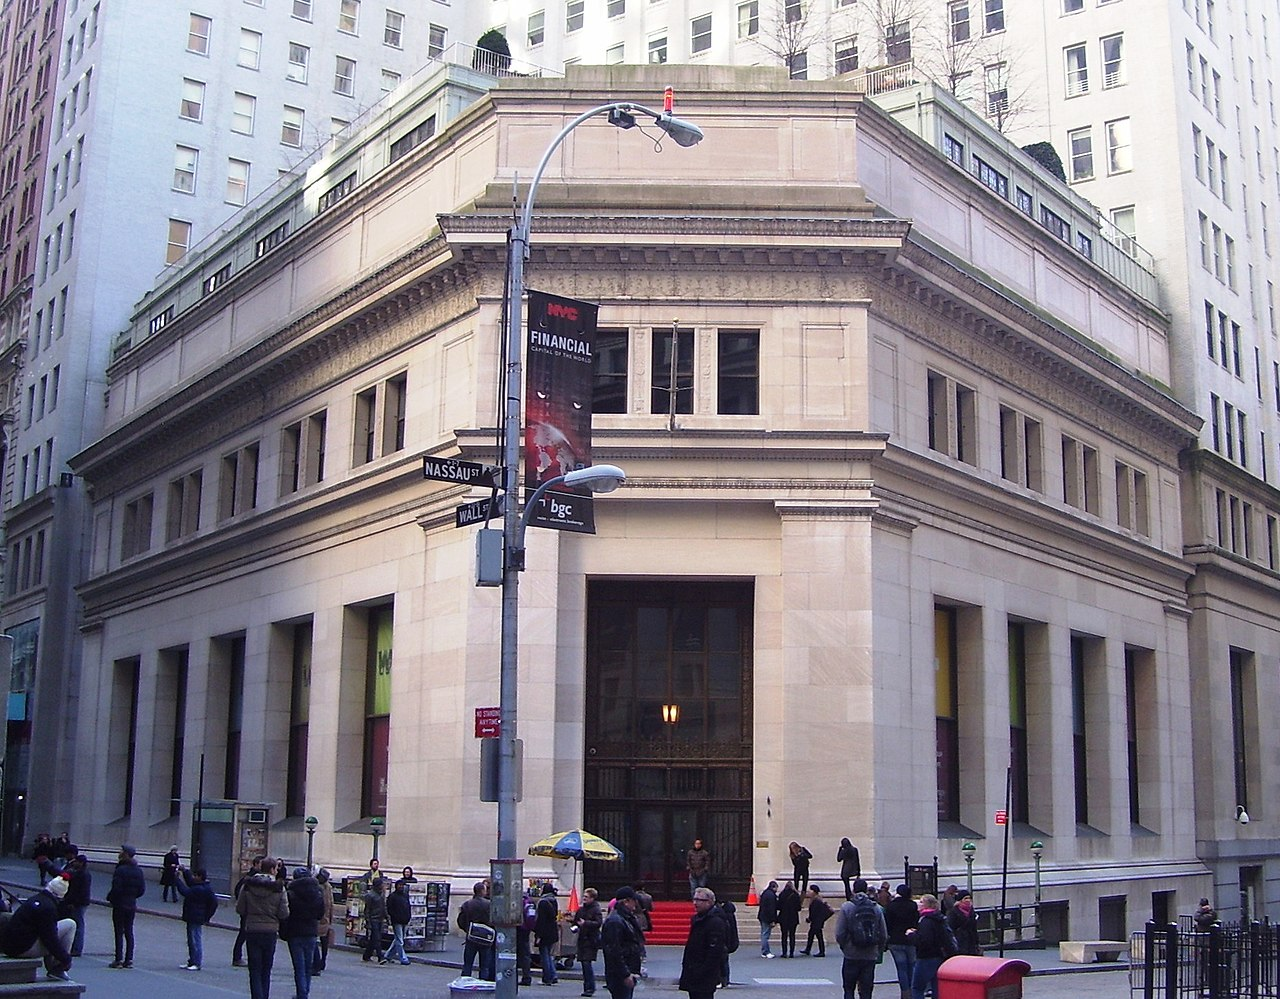
\includegraphics[height=0.40\textheight]{ch8_jpmorgan_23wall.jpg}\\[1mm]
\imgcap{The J.P. Morgan building at 23 Wall Street, New York}
\imgcredit{https://commons.wikimedia.org/wiki/File:J._P._Morgan_\%26_Company_Building_23_Wall_Street.jpg}{Photo: Beyond My Ken (2012); CC BY-SA 4.0; Wikimedia Commons}
\end{column}
\end{columns}
\end{frame}

\begin{frame}{From RiskMetrics to Basel}
\itemsize{\footnotesize}
\begin{columns}[T]
\begin{column}{0.58\textwidth}
\begin{itemize}
    \item The \textbf{BCBS} (Basel Committee on Banking Supervision) sits at the \textbf{BIS} (Bank for International Settlements) in Basel \refBCBSh
    \begin{itemize}
        \item 1996: banks may compute market-risk capital with their own VaR models \refBCBSa
        \item rule: VaR 1\% over 10 days, times a multiplier of at least 3; the multiplier grows when the model fails the backtest \refBCBSb
    \end{itemize}
    \item 2019: the \textbf{FRTB} (Fundamental Review of the Trading Book) \refFRTB
    \begin{itemize}
        \item capital from ES 2.5\% instead of VaR 1\% \refMAR; backtesting still counts VaR exceptions \refMARb
    \end{itemize}
\end{itemize}
\end{column}
\begin{column}{0.38\textwidth}
\centering
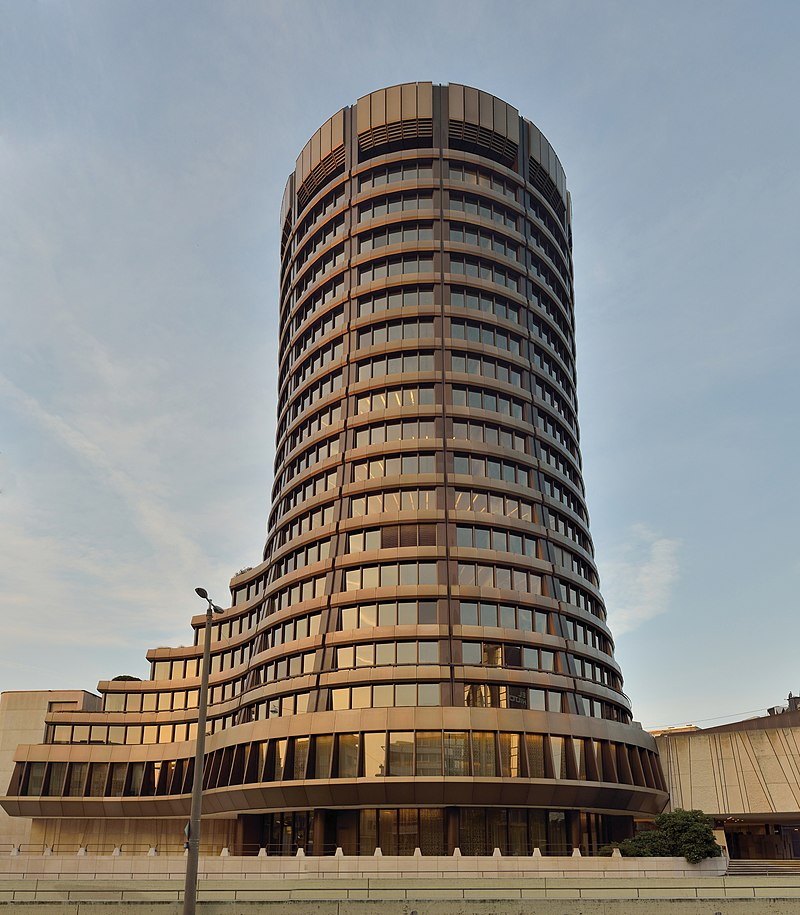
\includegraphics[height=0.42\textheight]{ch10_bis_tower_2014.jpg}\\[1mm]
\imgcap{The BIS tower in Basel, seat of the Basel Committee}
\imgcredit{https://commons.wikimedia.org/wiki/File:Basel_Committee_on_Banking_Supervision_-_BCBS.jpg}{Photo: Taxiarchos228 (2014); CC BY-SA 4.0; Wikimedia Commons}
\end{column}
\end{columns}
\end{frame}

\begin{frame}{Two Storms: 2008 and 2020}
\itemsize{\footnotesize}
\begin{columns}[T]
\begin{column}{0.48\textwidth}
\centering
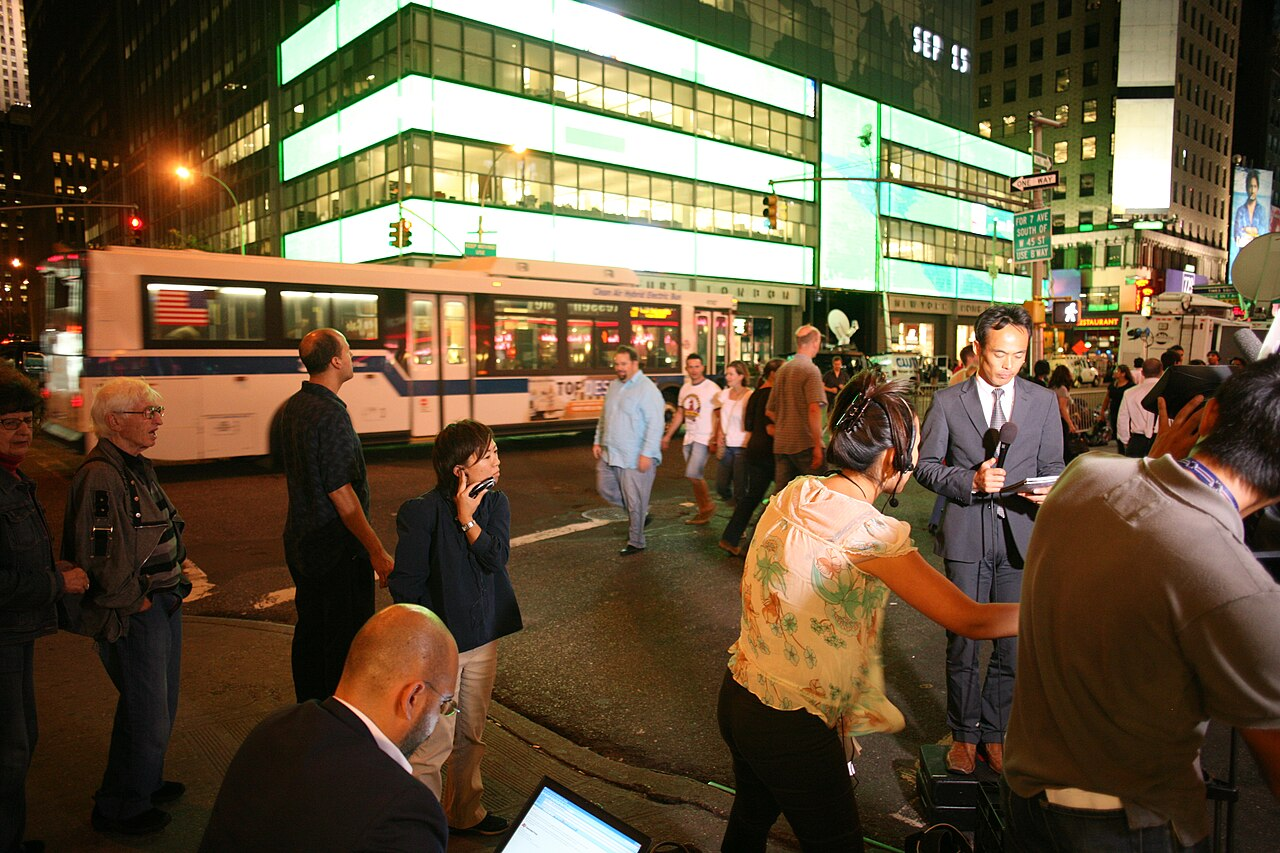
\includegraphics[height=0.30\textheight]{ch0_lehman_2008.jpg}\\[1mm]
\imgcap{Lehman Brothers headquarters, New York, 15 September 2008}
\imgcredit{https://commons.wikimedia.org/wiki/File:Lehman_Brothers-NYC-20080915.jpg}{Photo: Robert Scoble (2008); CC BY 2.0; Wikimedia Commons}
\end{column}
\begin{column}{0.48\textwidth}
\centering
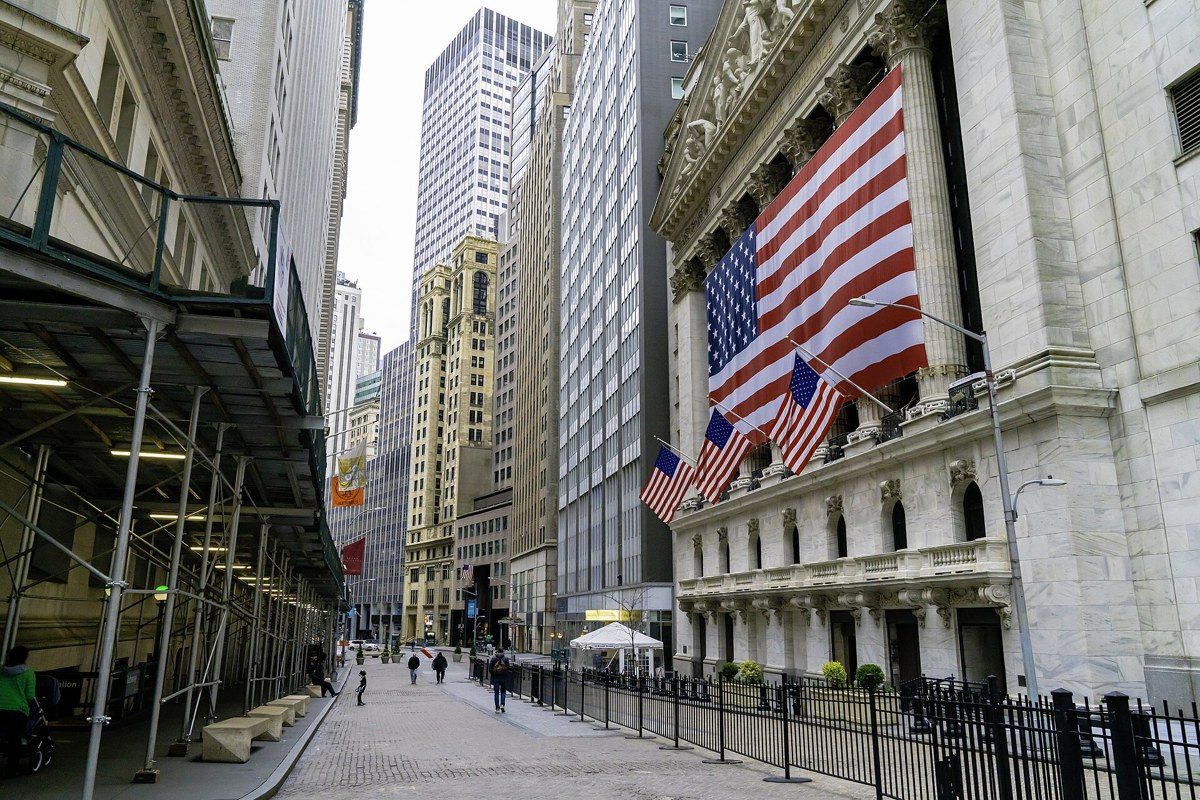
\includegraphics[height=0.30\textheight]{ch0_fidi_march_2020.jpg}\\[1mm]
\imgcap{The Financial District of New York, 25 March 2020}
\imgcredit{https://commons.wikimedia.org/wiki/File:Subdued_FiDi_(50063555551).jpg}{Photo: Billie Grace Ward (2020); CC BY 2.0; Wikimedia Commons}
\end{column}
\end{columns}\begin{itemize}
    \item The worst day of the S\&P 500 since 2000: $-12.8\%$ on 16 March 2020; a Normal model with the sample volatility gives such a day a probability of practically zero
    \item A risk measure must be judged in such periods: we use 2008 and 2020 as stress tests throughout the chapter
\end{itemize}
\end{frame}

\begin{frame}{Recap: Measuring Tail Risk}
\itemsize{\small}
\begin{itemize}
    \item VaR was born as a daily summary of the next day's loss (RiskMetrics, 1994)
    \item Basel: VaR 1\% for capital (1996), ES 2.5\% for capital and VaR 1\% for backtesting (FRTB, 2019)
    \item Crises are the real test of a risk model
\end{itemize}
\end{frame}


%=============================================================================
\section{VaR and ES: Definitions}
%=============================================================================

\begin{frame}{Losses, Horizon and Level}
\itemsize{\small}
\begin{itemize}
    \item $X$: the \textbf{P\&L} (profit and loss) or the return of a position over a horizon $h$ (here one day, in \%)
    \begin{itemize}
        \item the loss is $L = -X$: a positive number when the position loses money
    \end{itemize}
    \item The \textbf{level} $\alpha$ is the probability of the tail: $\alpha = 1\%$ or $\alpha = 2.5\%$
    \begin{itemize}
        \item we write \textbf{VaR 1\%} and \textbf{ES 2.5\%}: the bad outcomes have probability 1\% and 2.5\%
        \item the number in the name is always the tail probability: VaR 1\% is exceeded with probability 1\%
    \end{itemize}
    \item $q_\alpha(X) = \inf\{x : P(X \le x) > \alpha\}$: the $\alpha$-\textbf{quantile} of $X$ (\sfmchlink{https://danpele.github.io/SFM/EN/Courses/chapter2_classical_distributions_stylised_facts.pdf}{Chapter 2})
    \begin{itemize}
        \item for a continuous distribution function $F$: $q_\alpha = F^{-1}(\alpha)$, a negative number for small $\alpha$
    \end{itemize}
\end{itemize}
\end{frame}

\begin{frame}{Value at Risk}
\itemsize{\small}
\begin{itemize}
    \item \textbf{Definition}: $\mathrm{VaR}_\alpha(X) = -q_\alpha(X)$
    \begin{itemize}
        \item the loss that is exceeded with probability $\alpha$: $P(L > \mathrm{VaR}_\alpha) \le \alpha$
        \item the minus sign makes VaR a positive loss; a VaR of 3\% means ``a loss of more than 3\% happens on 1 day in 100''
    \end{itemize}
    \item What VaR does \textbf{not} say
    \begin{itemize}
        \item how large the loss is on the bad days: a loss of 4\% and a loss of 40\% beyond VaR give the same VaR
        \item VaR is not the maximum loss: by construction it is exceeded on about $\alpha$ of the days
    \end{itemize}
    \item In money: a position of value $W$ has $\mathrm{VaR} = W \times \mathrm{VaR}(\%)/100$
\end{itemize}
\end{frame}

\begin{frame}{Expected Shortfall}
\itemsize{\small}
\begin{itemize}
    \item \textbf{Definition}: $\mathrm{ES}_\alpha(X) = -\dfrac{1}{\alpha}\displaystyle\int_0^\alpha q_u(X)\,du$: the average of the VaRs at all levels below $\alpha$
    \begin{itemize}
        \item for a continuous distribution: $\mathrm{ES}_\alpha = -E[X \mid X \le q_\alpha(X)]$, the average loss on the worst $\alpha$ of the days
        \item $u$: the integration variable, a tail level running from 0 to $\alpha$
        \item other names: CVaR (conditional VaR), TVaR (tail VaR), expected tail loss
    \end{itemize}
    \item Properties
    \begin{itemize}
        \item $\mathrm{ES}_\alpha \ge \mathrm{VaR}_\alpha$ at the same level $\alpha$
        \item ES looks inside the tail: two distributions with the same VaR but different tails have different ES
    \end{itemize}
\end{itemize}
\end{frame}

\begin{frame}{Worked Example: VaR and ES from 100 Days}
\itemsize{\small}
\begin{itemize}
    \item A position has 100 daily returns; the five worst are $-6.1$, $-4.8$, $-4.2$, $-3.9$, $-3.5$ (in \%)
    \begin{itemize}
        \item empirical quantile at level $\alpha$: the $k$-th smallest return, $k = \lceil n\alpha \rceil$ ($\lceil\cdot\rceil$: rounding up)
    \end{itemize}
    \item \textbf{VaR 1\%}: $k = \lceil 100 \times 0.01 \rceil = 1$, so $\mathrm{VaR}_{1\%} = 6.1\%$
    \begin{itemize}
        \item one observation decides VaR 1\%: with 100 days the estimate is very imprecise
    \end{itemize}
    \item \textbf{ES 2.5\%}: $k = \lceil 2.5 \rceil = 3$; the average of the three worst losses
    \begin{itemize}
        \item $\mathrm{ES}_{2.5\%} = (6.1 + 4.8 + 4.2)/3 = 5.03\%$; $\mathrm{VaR}_{2.5\%} = 4.2\%$
    \end{itemize}
    \item A position of 1 million RON: VaR 1\% = 61\,000 RON; on one day in a hundred the loss is larger
\end{itemize}
\end{frame}

\begin{frame}{VaR 1\% and ES 2.5\% of the S\&P 500}
\itemsize{\footnotesize}
\begin{center}
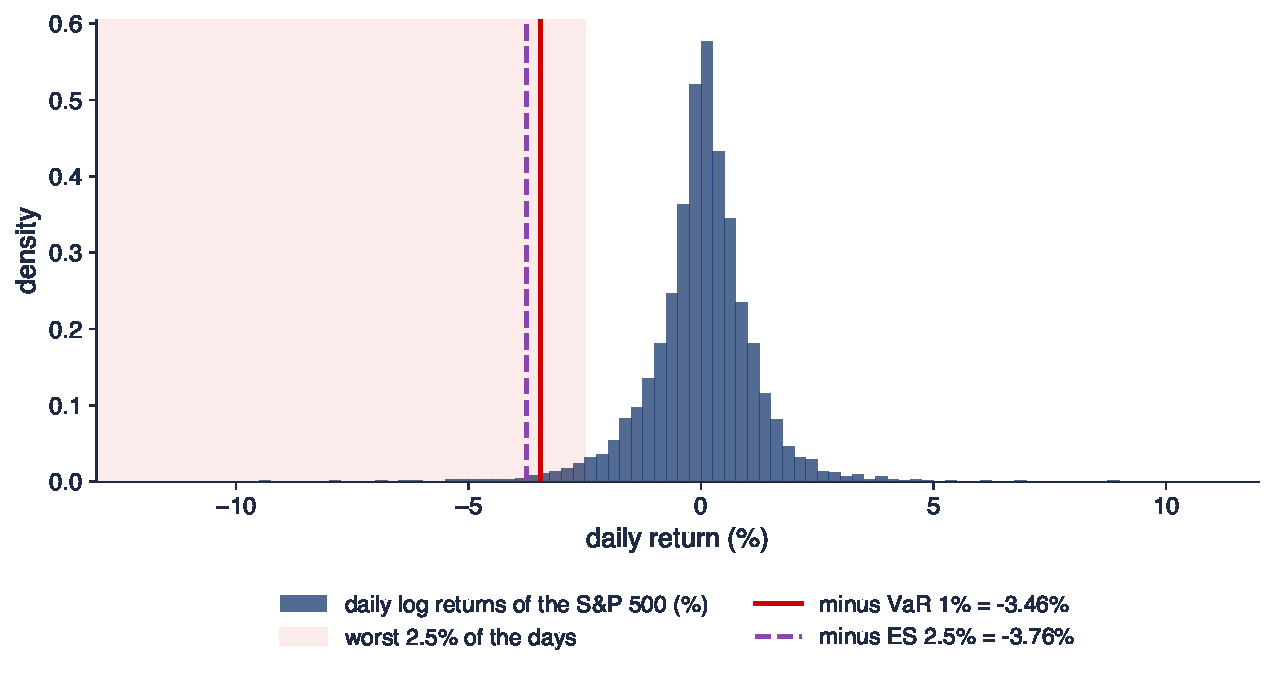
\includegraphics[width=0.97\textwidth,height=0.50\textheight,keepaspectratio]{sfm_ch10_var_es_def.pdf}
\end{center}
\vspace{-0.25cm}
\begin{itemize}
    \item Daily log returns since 2000 (6\,714 days); historical estimates: VaR 1\% $= 3.46\%$, VaR 2.5\% $= 2.51\%$, ES 2.5\% $= 3.76\%$
    \item Interpretation: ES 2.5\% averages the whole shaded tail, including the extreme days of 2008 and 2020; VaR 1\% is one point in that tail
    \item For a position of 1 million RON in the index: VaR 1\% about 34\,552 RON, ES 2.5\% about 37\,613 RON
\end{itemize}
\sfmquantlet{Ch_10}{SFM_ch10_var_methods}
\end{frame}

\begin{frame}{The Normal Distribution: Closed Forms}
\itemsize{\footnotesize}
\begin{itemize}
    \item $X \sim N(\mu, \sigma^2)$, $z_\alpha = \Phi^{-1}(\alpha)$ ($\Phi$, $\varphi$: distribution function and density of $N(0,1)$)
    \begin{itemize}
        \item $\mathrm{VaR}_\alpha = -(\mu + \sigma z_\alpha)$, \quad $\mathrm{ES}_\alpha = -\mu + \sigma\,\dfrac{\varphi(z_\alpha)}{\alpha}$
        \item derivation: $E[Z \mid Z \le z] = -\varphi(z)/\Phi(z)$ because $\varphi'(z) = -z\varphi(z)$
    \end{itemize}
    \item Numbers: $z_{0.01} = -2.326$; $z_{0.025} = -1.960$, $\varphi(z_{0.025}) = 0.0584$, $\varphi(z_{0.025})/0.025 = 2.338$
    \begin{itemize}
        \item ES 2.5\% / VaR 1\% $= 2.338/2.326 = 1.005$ (with $\mu = 0$): for Normal returns the two measures are almost equal
        \item this is why ES 2.5\% replaced VaR 1\% in Basel: same size for Normal data, larger for heavy tails
    \end{itemize}
\end{itemize}
\end{frame}

\begin{frame}{Worked Example: Normal VaR and ES of the S\&P 500}
\itemsize{\small}
\begin{itemize}
    \item Sample moments of the daily returns since 2000: $\hat\mu = 0.025$, $\hat\sigma = 1.21$ (in \%)
    \begin{itemize}
        \item VaR 1\% $= -(0.025 - 2.326 \times 1.21) = -0.025 + 2.822 = 2.80\%$
        \item ES 2.5\% $= -0.025 + 2.338 \times 1.21 = -0.025 + 2.836 = 2.81\%$
    \end{itemize}
    \item Compare with the data (historical simulation): VaR 1\% $= 3.46\%$, ES 2.5\% $= 3.76\%$
    \begin{itemize}
        \item the Normal VaR 1\% is 19\% too low: the Normal tail is too thin (\sfmchlink{https://danpele.github.io/SFM/EN/Courses/chapter2_classical_distributions_stylised_facts.pdf}{Chapter 2})
        \item the Normal ES 2.5\% is even further from the data: it ignores the extreme days
    \end{itemize}
    \item Interpretation: two parameters cannot describe the tail; the next methods change either the distribution or the data used
\end{itemize}
\end{frame}

\begin{frame}{The Student-t Distribution: Closed Forms}
\itemsize{\footnotesize}
\begin{itemize}
    \item $X = m + s\,T$, $T \sim t_\nu$ (location $m$, scale $s$, $\nu$ degrees of freedom, \sfmchlink{https://danpele.github.io/SFM/EN/Courses/chapter2_classical_distributions_stylised_facts.pdf}{Chapter 2}); $t_\alpha = t_\nu^{-1}(\alpha)$, $f_\nu$ the density of $t_\nu$
    \begin{itemize}
        \item $\mathrm{VaR}_\alpha = -(m + s\,t_\alpha)$, \quad $\mathrm{ES}_\alpha = -m + s\,\dfrac{f_\nu(t_\alpha)}{\alpha}\,\dfrac{\nu + t_\alpha^2}{\nu - 1}$ (for $\nu > 1$)
        \item the variance is $s^2\nu/(\nu - 2)$: a \textbf{standardised} t (variance 1) has $s = \sqrt{(\nu - 2)/\nu}$
    \end{itemize}
    \item \textbf{Worked example}: S\&P 500, maximum likelihood: $\hat m = 0.068$, $\hat s = 0.703$, $\hat\nu = 2.67$
    \begin{itemize}
        \item $t_{0.01} = -5.023$: VaR 1\% $= -(0.068 + 0.703 \times (-5.023)) = 3.46\%$
        \item ES factor $5.720$: ES 2.5\% $= -0.068 + 0.703 \times 5.720 = 3.95\%$
    \end{itemize}
    \item Interpretation: with $\nu < 3$ the fitted tail is very heavy: VaR 1\% matches the data, ES 2.5\% is above the historical $3.76\%$
\end{itemize}
\end{frame}

\begin{frame}{From One Day to Ten Days}
\itemsize{\footnotesize}
\begin{itemize}
    \item \textbf{Square-root-of-time rule}: $\mathrm{VaR}^{(h)} \approx \sqrt{h}\,\mathrm{VaR}^{(1)}$
    \begin{itemize}
        \item exact for i.i.d.\ Normal returns with mean 0: the $h$-day return has standard deviation $\sigma\sqrt{h}$
        \item Basel 1996: 10-day VaR, usually scaled from one day with $\sqrt{10} = 3.162$
    \end{itemize}
    \item S\&P 500, historical simulation
    \begin{itemize}
        \item one day: 3.46\%; scaled: $3.162 \times 3.46 = 10.93\%$
        \item VaR 1\% of overlapping 10-day returns: 10.37\%
    \end{itemize}
    \item Why the rule fails in general
    \begin{itemize}
        \item heavy tails: a sum of 10 heavy-tailed returns is closer to Normal (CLT, central limit theorem), so the ratio of quantiles is below $\sqrt{10}$
        \item volatility clustering: after a calm day the 10-day risk is larger than $\sqrt{10}$ times today's, after a storm smaller (\sfmchlink{https://danpele.github.io/SFM/EN/Courses/chapter9_arch_garch_models.pdf}{Chapter 9})
    \end{itemize}
\end{itemize}
\end{frame}

\begin{frame}{Recap: Definitions of VaR and ES}
\itemsize{\small}
\begin{itemize}
    \item $\mathrm{VaR}_\alpha = -q_\alpha$: the loss exceeded with probability $\alpha$; $\mathrm{ES}_\alpha$: the average loss beyond it
    \item Normal: ES 2.5\% $\approx$ VaR 1\%; heavy tails make ES 2.5\% larger
    \item Scaling to 10 days by $\sqrt{10}$ is a convention, not a law
\end{itemize}
\end{frame}


%=============================================================================
\section{Coherent Risk Measures}
%=============================================================================

\begin{frame}{1999: Four Axioms for a Risk Measure}
\itemsize{\footnotesize}
\begin{columns}[T]
\begin{column}{0.64\textwidth}
\begin{itemize}
    \item \refArtzner: a risk measure $\rho$ maps a loss $L$ to the capital that makes it acceptable; $\rho$ is \textbf{coherent} if
    \begin{itemize}
        \item \textbf{monotonicity}: $L_1 \le L_2$ always $\Rightarrow \rho(L_1) \le \rho(L_2)$
        \item \textbf{translation invariance}: $\rho(L + c) = \rho(L) + c$ for a sure amount $c$
        \item \textbf{positive homogeneity}: $\rho(\lambda L) = \lambda\rho(L)$, $\lambda > 0$
        \item \textbf{subadditivity}: $\rho(L_1 + L_2) \le \rho(L_1) + \rho(L_2)$
    \end{itemize}
    \item Subadditivity: diversification never adds risk; a bank can add the capital of its desks as an upper bound
\end{itemize}
\end{column}
\begin{column}{0.32\textwidth}
\centering

\includegraphics[height=0.40\textheight]{ch10_delbaen_1997.jpg}\\[1mm]
\imgcap{Freddy Delbaen, co-author of the axioms (1997)}
\imgcredit{https://commons.wikimedia.org/wiki/File:ETH-BIB-Delbaen,_Freddy_(1946-)-Portr_16468.tif}{Photo: ETH-Bibliothek Zürich, Bildarchiv (1997); CC BY-SA 4.0; Wikimedia Commons}
\end{column}
\end{columns}
\end{frame}

\begin{frame}{Counterexample: Two Bonds, Step by Step}
\itemsize{\footnotesize}
\begin{itemize}
    \item Two independent bonds; each loses 100 with probability 4\% (default) and 0 otherwise; level $\alpha = 5\%$
    \begin{itemize}
        \item one bond: $P(L > 0) = 4\% \le 5\%$, so $\mathrm{VaR}_{5\%} = 0$ for each
    \end{itemize}
    \item Both bonds: $P(L = 200) = 0.16\%$, $P(L = 100) = 7.68\%$, so $P(L > 0) = 7.84\% > 5\%$
    \begin{itemize}
        \item $\mathrm{VaR}_{5\%}(L_1 + L_2) = 100 > 0 + 0$: VaR \textbf{punishes} diversification
    \end{itemize}
    \item ES 5\% (the average of the worst 5\% of outcomes)
    \begin{itemize}
        \item one bond: $(4\% \times 100 + 1\% \times 0)/5\% = 80$
        \item both: $(0.16\% \times 200 + (5 - 0.16)\% \times 100)/5\% = 103.2 \le 80 + 80$: subadditive
    \end{itemize}
\end{itemize}
\end{frame}

\begin{frame}{ES Is Coherent; VaR Only Sometimes}
\itemsize{\small}
\begin{itemize}
    \item \textbf{ES} satisfies all four axioms \refAT
    \begin{itemize}
        \item reason: ES is an average of quantiles over the tail, and averaging respects sums
    \end{itemize}
    \item \textbf{VaR} satisfies the first three; subadditivity can fail
    \begin{itemize}
        \item fails for discrete losses (credit, the bonds above) and for extremely heavy tails (tail index below 1, \sfmchlink{https://danpele.github.io/SFM/EN/Courses/chapter5_heavy_tails_evt.pdf}{Chapter 5})
        \item holds for elliptical distributions (Normal, Student-t) and, in practice, for most equity returns \refDJSS
    \end{itemize}
    \item ES needs a finite mean of the losses; VaR always exists
\end{itemize}
\end{frame}

\begin{frame}{Elicitability: Can a Forecast Be Scored?}
\itemsize{\small}
\begin{itemize}
    \item A statistic is \textbf{elicitable} if some loss (scoring) function is minimised, on average, by its true value \refGneiting
    \begin{itemize}
        \item the mean: squared error; the median: absolute error
    \end{itemize}
    \item \textbf{VaR is elicitable}: the quantile (pinball) loss $S(v, x) = (\alpha - \mathbf{1}\{x < -v\})(x + v)$
    \begin{itemize}
        \item $v$: the VaR forecast; $x$: the realised return; $\mathbf{1}\{\cdot\}$: 1 if the event occurs, 0 otherwise
        \item two VaR models can be compared by their average quantile loss
    \end{itemize}
    \item \textbf{ES alone is not elicitable} \refGneiting; the pair (VaR, ES) is \refFZ
    \begin{itemize}
        \item consequence: ES forecasts are tested together with VaR forecasts (Section 7)
    \end{itemize}
\end{itemize}
\end{frame}

\begin{frame}{Recap: Coherent Risk Measures}
\itemsize{\small}
\begin{itemize}
    \item Coherence: monotonicity, translation invariance, positive homogeneity, subadditivity
    \item ES is coherent; VaR can penalise diversification (two bonds)
    \item VaR is elicitable, ES only together with VaR
\end{itemize}
\end{frame}


%=============================================================================
\section{Estimating VaR and ES}
%=============================================================================

\begin{frame}{Five Unconditional Methods at a Glance}
\itemsize{\footnotesize}
\begin{center}
\footnotesize
\begin{tabular}{>{\raggedright\arraybackslash}p{2.3cm}>{\raggedright\arraybackslash}p{4.0cm}>{\raggedright\arraybackslash}p{4.6cm}}
\toprule
\textbf{Method} & \textbf{Assumption} & \textbf{Weak point} \\
\midrule
historical simulation (HS) & the past window is a sample of tomorrow & few tail points; nothing beyond the worst day \\
Normal & returns are Normal & tails far too thin \\
Student-t & returns are Student-t & one tail shape for both tails \\
Cornish--Fisher & Normal quantile corrected by skewness and kurtosis & breaks down for large kurtosis \\
EVT (POT) & GPD above a high threshold (\sfmchlink{https://danpele.github.io/SFM/EN/Courses/chapter5_heavy_tails_evt.pdf}{Chapter 5}) & choice of the threshold \\
\bottomrule
\end{tabular}
\end{center}
\begin{itemize}
    \item ``Unconditional'': the same VaR every day of the window; conditional methods (Section 5) use today's volatility
    \item All methods: daily log returns in \% (\sfmchlink{https://danpele.github.io/SFM/EN/Courses/chapter1_data_returns_indicators.pdf}{Chapter 1}), VaR and ES as positive losses
\end{itemize}
\end{frame}

\begin{frame}{Historical Simulation}
\itemsize{\small}
\begin{itemize}
    \item \textbf{Algorithm}: take the last $n$ returns $r_{t-n+1}, \dots, r_t$, sort them: $r_{(1)} \le \dots \le r_{(n)}$
    \begin{itemize}
        \item $\widehat{\mathrm{VaR}}_\alpha = -r_{(k)}$, $k = \lceil n\alpha \rceil$; \quad $\widehat{\mathrm{ES}}_\alpha = -\frac{1}{k}\sum_{i=1}^{k} r_{(i)}$
        \item no distribution is assumed: the empirical distribution of the window is the forecast
    \end{itemize}
    \item Ported from the SFE Quantlet VaRest
\end{itemize}
\end{frame}

\begin{frame}{Worked Example: Historical Simulation on the S\&P 500}
\itemsize{\footnotesize}
\begin{itemize}
    \item S\&P 500 since 2000: $n = 6\,714$
    \begin{itemize}
        \item VaR 1\%: $k = \lceil 67.14 \rceil = 68$, the 68-th worst day: $3.46\%$
        \item ES 2.5\%: the average of the $\lceil 167.85 \rceil = 168$ worst days: $3.76\%$
    \end{itemize}
    \item The window $n$ is a trade-off
    \begin{itemize}
        \item short (250 days): reacts, but VaR 1\% rests on 3 observations; long (all data): stable, but blind to today's volatility
        \item \textbf{ghost effect}: a crash day changes VaR when it enters the window and again, abruptly, $n$ days later when it leaves
    \end{itemize}
\end{itemize}
\end{frame}

\begin{frame}{How Precise Is a Historical VaR?}
\itemsize{\footnotesize}
\begin{itemize}
    \item A VaR estimate is a statistic: it has a sampling error; we measure it with the bootstrap (\sfmchlink{https://danpele.github.io/SFM/EN/Courses/chapter2_classical_distributions_stylised_facts.pdf}{Chapter 2})
    \begin{itemize}
        \item resample the $n$ returns with replacement 2000 times, recompute VaR and ES, read the 2.5\% and 97.5\% quantiles
    \end{itemize}
    \item S\&P 500, all 6\,714 days: VaR 1\% $= 3.46\%$, 95\% interval [3.18, 3.66]; ES 2.5\% $= 3.76\%$, [3.46, 4.07]
    \begin{itemize}
        \item last 500 days: VaR 1\% $= 2.75\%$, [1.99, 4.96]; ES 2.5\% $= 2.94\%$, [2.14, 3.82]
    \end{itemize}
    \item With two years of data the interval of VaR 1\% is wider than 2 percentage points: VaR 1\% rests on 5 observations
    \item Interpretation: differences between methods smaller than the bootstrap interval are not evidence that one method is better
\end{itemize}\sfmquantlet{Ch_10}{SFM_ch10_var_methods}
\end{frame}

\begin{frame}{The Cornish--Fisher Expansion}
\itemsize{\footnotesize}
\begin{itemize}
    \item \refCF: correct the Normal quantile $z = z_\alpha$ with the skewness $S$ and the excess kurtosis $K$ (kurtosis minus 3)
    \begin{itemize}
        \item $z_{CF} = z + \dfrac{(z^2 - 1)S}{6} + \dfrac{(z^3 - 3z)K}{24} - \dfrac{(2z^3 - 5z)S^2}{36}$, \quad $\mathrm{VaR}_\alpha = -(\mu + \sigma z_{CF})$
        \item negative $S$ and positive $K$ push the quantile further into the left tail
    \end{itemize}
    \item S\&P 500: $S = -0.35$, $K = 10.7$, $z_{0.01} = -2.326$
    \begin{itemize}
        \item $z_{CF} = -5.03$, so VaR 1\% $= 6.08\%$, against the historical $3.46\%$
    \end{itemize}
    \item Interpretation: the expansion is a small correction around the Normal; with an excess kurtosis above 10 it overshoots badly
    \begin{itemize}
        \item use it only when $|S|$ and $K$ are moderate (for example monthly returns or diversified portfolios)
    \end{itemize}
\end{itemize}
\end{frame}

\begin{frame}{EVT: Peaks over Threshold (\sfmchlinkt{https://danpele.github.io/SFM/EN/Courses/chapter5_heavy_tails_evt.pdf}{Chapter 5})}
\itemsize{\footnotesize}
\begin{itemize}
    \item Losses $L = -r$; threshold $u$ = the 90\% quantile of the losses \refMF; excesses $L - u$ above $u$ follow a GPD (generalised Pareto distribution) with shape $\xi$ and scale $\beta$
    \begin{itemize}
        \item $\mathrm{VaR}_\alpha = u + \dfrac{\beta}{\xi}\Big[\Big(\dfrac{n\alpha}{N_u}\Big)^{-\xi} - 1\Big]$, \quad $\mathrm{ES}_\alpha = \dfrac{\mathrm{VaR}_\alpha + \beta - \xi u}{1 - \xi}$ ($N_u$: number of excesses)
        \item $n$: the number of days; $n\alpha/N_u$: the tail probability relative to the share of excesses; $\xi > 0$: a heavy tail
    \end{itemize}
    \item S\&P 500: $u = 1.26\%$, $N_u = 672$ (10.0\% of the days), $\hat\xi = 0.164$, $\hat\beta = 0.820$
    \begin{itemize}
        \item VaR 1\%: $n\alpha/N_u = 0.0999$, $0.0999^{-\hat\xi} = 1.461$; $\hat\beta/\hat\xi = 4.988$; $1.26 + 4.988 \times (1.461 - 1) = 3.56\%$
        \item ES 2.5\% $= 3.77\%$; $\hat\xi > 0$: a heavy (Pareto-type) tail
    \end{itemize}
    \item EVT smooths the tail and extrapolates beyond the worst observed day: useful for VaR 0.1\% and for stress tests
\end{itemize}
\end{frame}

\begin{frame}{VaR across Tail Probabilities}
\itemsize{\footnotesize}
\begin{center}
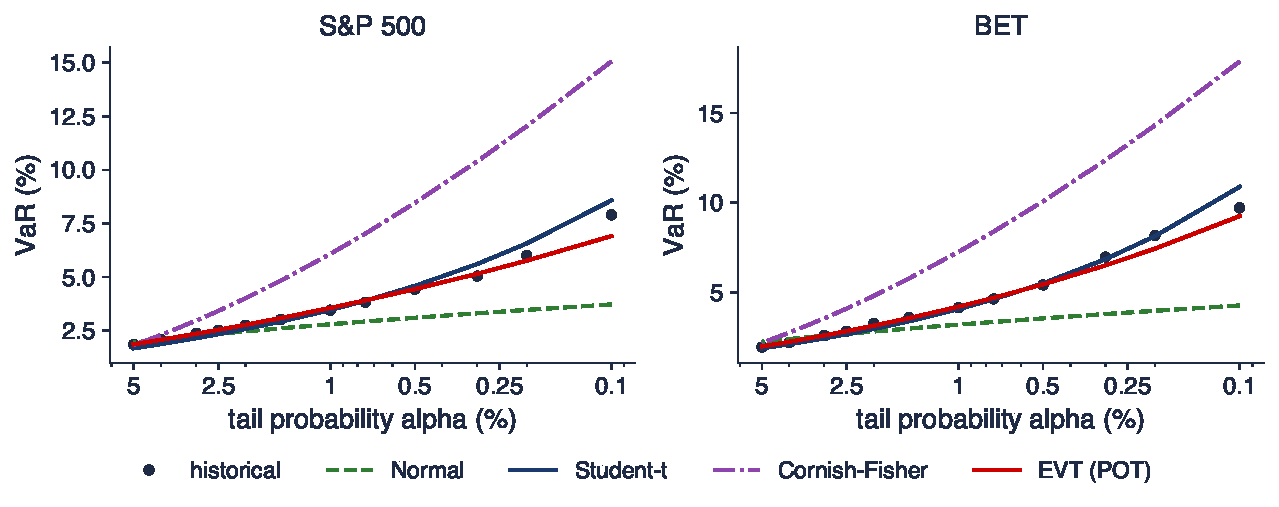
\includegraphics[width=0.97\textwidth,height=0.52\textheight,keepaspectratio]{sfm_ch10_var_curves.pdf}
\end{center}
\vspace{-0.25cm}
\begin{itemize}
    \item Each line: $\mathrm{VaR}_\alpha$ of one method for $\alpha$ from 5\% to 0.1\%; points: historical simulation
    \item Interpretation: at 5\% all methods agree; at 1\% the Normal is too low; at 0.1\% Student-t and EVT stay close to the data, while Cornish--Fisher explodes
\end{itemize}
\sfmquantlet{Ch_10}{SFM_ch10_var_methods}
\end{frame}

\begin{frame}{VaR 1\% by Method on Six Series}
\itemsize{\footnotesize}
\begin{center}
\footnotesize
\begin{tabular}{lrrrrrrr}
\toprule
& HS & Normal & Student-t & Cornish--Fisher & EVT & $K$ & $\hat\xi$ \\
\midrule
S\&P 500 & $3.46$ & $2.80$ & $3.46$ & $6.08$ & $3.56$ & ${10.7}$ & $0.16$ \\
DAX & $4.20$ & $3.26$ & $3.96$ & $5.42$ & $4.05$ & ${6.1}$ & $0.12$ \\
BET & $4.14$ & $3.19$ & $4.06$ & $7.25$ & $4.19$ & ${11.1}$ & $0.23$ \\
Bitcoin & $10.54$ & $7.99$ & $11.06$ & $18.89$ & $10.38$ & ${12.0}$ & $0.12$ \\
TLV & $5.11$ & $4.01$ & $4.63$ & $10.19$ & $4.90$ & ${13.5}$ & $0.26$ \\
SNP & $4.29$ & $3.70$ & $4.26$ & $7.55$ & $4.38$ & ${8.9}$ & $0.22$ \\
\bottomrule
\end{tabular}
\end{center}
\begin{itemize}
    \item Whole samples (S\&P 500, DAX, BET since 2000; Bitcoin since 2014; TLV and SNP since 2010), in \%; $K$: excess kurtosis
    \item HS, Student-t and EVT differ by at most 0.7 percentage points; the Normal VaR is 14--24\% too low everywhere
    \item Cornish--Fisher gives 1.3 to 2.0 times the historical VaR: with $K$ between 6 and 14 the expansion is outside its range
\end{itemize}\sfmquantlet{Ch_10}{SFM_ch10_var_methods}
\end{frame}

\begin{frame}{ES 2.5\% by Method on Six Series}
\itemsize{\footnotesize}
\begin{center}
\footnotesize
\begin{tabular}{lrrrrrrr}
\toprule
& HS & Normal & Student-t & Cornish--Fisher & EVT & $K$ & $\hat\xi$ \\
\midrule
S\&P 500 & $3.76$ & $2.81$ & $3.95$ & $6.65$ & $3.77$ & ${10.7}$ & $0.16$ \\
DAX & $4.26$ & $3.27$ & $4.37$ & $5.81$ & $4.24$ & ${6.1}$ & $0.12$ \\
BET & $4.57$ & $3.21$ & $4.76$ & $7.93$ & $4.57$ & ${11.1}$ & $0.23$ \\
Bitcoin & $10.84$ & $8.03$ & $13.37$ & $20.69$ & $10.90$ & ${12.0}$ & $0.12$ \\
TLV & $5.37$ & $4.03$ & $5.03$ & $11.20$ & $5.35$ & ${13.5}$ & $0.26$ \\
SNP & $4.70$ & $3.72$ & $4.57$ & $8.18$ & $4.71$ & ${8.9}$ & $0.22$ \\
\bottomrule
\end{tabular}
\end{center}
\begin{itemize}
    \item Normal: ES 2.5\% equals its VaR 1\%; the data: the historical ES 2.5\% is 1.5--10.5\% above the historical VaR 1\%
    \item For the S\&P 500, DAX, BET and Bitcoin, Student-t gives the largest ES among the sensible methods (Bitcoin: $13.37\%$ against $10.84\%$): with $\hat\nu < 3$ its tail is heavier than the data beyond the threshold
    \item Interpretation: EVT and HS agree at 2.5\%; the method matters more for ES than for VaR, because ES depends on the whole tail
\end{itemize}\sfmquantlet{Ch_10}{SFM_ch10_var_methods}
\end{frame}

\begin{frame}{Recap: Estimating VaR and ES}
\itemsize{\small}
\begin{itemize}
    \item HS: sorted window; Normal and Student-t: closed forms; Cornish--Fisher: moment correction; EVT: GPD tail
    \item On daily data: Normal too low, Cornish--Fisher too high, HS, Student-t and EVT close at 1\%
    \item All five ignore today's volatility
\end{itemize}
\end{frame}


%=============================================================================
\section{Conditional VaR: GARCH and Filtered Historical Simulation}
%=============================================================================

\begin{frame}{Why Condition on Today's Volatility?}
\itemsize{\footnotesize}
\begin{itemize}
    \item Volatility clustering (\sfmchlink{https://danpele.github.io/SFM/EN/Courses/chapter8_volatility_estimators.pdf}{Chapters 8} and \sfmchlink{https://danpele.github.io/SFM/EN/Courses/chapter9_arch_garch_models.pdf}{9}): a calm day is followed by calm days, a storm by storms
    \begin{itemize}
        \item an unconditional VaR is too high in calm years and too low at the start of a crisis
    \end{itemize}
    \item Conditional model: $r_{t+1} = \mu + \sigma_{t+1}z_{t+1}$, $z$ i.i.d.\ with mean 0 and variance 1
    \begin{itemize}
        \item $\mathrm{VaR}_{t+1} = -(\mu + \sigma_{t+1}\,q_\alpha(z))$, \quad $\mathrm{ES}_{t+1} = -\mu + \sigma_{t+1}\,\mathrm{ES}_\alpha(z)$
        \item $q_\alpha(z)$, $\mathrm{ES}_\alpha(z)$: the quantile and the ES of the standardised innovation $z$
        \item two ingredients: the volatility forecast $\sigma_{t+1}$ and the distribution of $z$
    \end{itemize}
    \item Two choices for the distribution of $z$
    \begin{itemize}
        \item \textbf{GARCH-t}: standardised Student-t with $\nu$ estimated with the GARCH(1,1) \refBoll
        \item \textbf{FHS} (filtered historical simulation): the empirical distribution of the standardised residuals $\hat z_t = (r_t - \hat\mu)/\hat\sigma_t$ \refHW; \refBGV
    \end{itemize}
\end{itemize}
\end{frame}

\begin{frame}{Worked Example: the S\&P 500 on 18 September 2026}
\itemsize{\footnotesize}
\begin{itemize}
    \item GARCH(1,1)-t on all data: $\hat\mu = 0.079$, $\hat\alpha = 0.123$, $\hat\beta = 0.872$, $\hat\nu = 6.26$; forecast for the next day $\sigma_{t+1} = 0.714\%$
    \item \textbf{GARCH-t}: $q_{0.01}(z) = t_\nu^{-1}(0.01)\sqrt{(\nu - 2)/\nu} = -2.557$; $\mathrm{ES}_{2.5\%}(z) = 2.644$
    \begin{itemize}
        \item VaR 1\% $= -(0.079 + 0.714 \times (-2.557)) = 1.75\%$; ES 2.5\% $= -0.079 + 0.714 \times 2.644 = 1.81\%$
    \end{itemize}
    \item \textbf{FHS}: the 1\% quantile of the 6\,714 standardised residuals is $-2.787$; their ES 2.5\% is $2.952$
    \begin{itemize}
        \item VaR 1\% $= -(0.079 + 0.714 \times (-2.787)) = 1.91\%$; ES 2.5\% $= 2.03\%$
    \end{itemize}
    \item Interpretation: a calm market: the conditional VaR 1\% is about half of the unconditional $3.46\%$; the standardised residuals have a heavier left tail than the fitted t
\end{itemize}\sfmquantlet{Ch_10}{SFM_ch10_conditional_var}
\end{frame}

\begin{frame}{Next-Day VaR and ES on Six Series}
\itemsize{\footnotesize}
\begin{center}
\footnotesize
\begin{tabular}{lrrrrrrr}
\toprule
& \multicolumn{3}{c}{VaR 1\%} & \multicolumn{3}{c}{ES 2.5\%} & \\ & HS (all) & GARCH-t & FHS & HS (all) & GARCH-t & FHS & $\sigma_{t+1}$ \\
\midrule
S\&P 500 & $3.46$ & $1.75$ & $1.91$ & $3.76$ & $1.81$ & $2.03$ & $0.714$ \\
DAX & $4.20$ & $2.31$ & $2.48$ & $4.26$ & $2.38$ & $2.55$ & $0.945$ \\
BET & $4.14$ & $4.51$ & $4.81$ & $4.57$ & $4.72$ & $5.04$ & $1.763$ \\
Bitcoin & $10.54$ & $7.37$ & $7.99$ & $10.84$ & $8.11$ & $8.57$ & $2.829$ \\
TLV & $5.11$ & $7.18$ & $7.33$ & $5.37$ & $7.53$ & $8.00$ & $2.791$ \\
SNP & $4.29$ & $5.06$ & $5.39$ & $4.70$ & $5.31$ & $5.65$ & $1.966$ \\
\bottomrule
\end{tabular}
\end{center}
\begin{itemize}
    \item Forecasts for the day after 18 September 2026, in \%; HS (all): the unconditional historical values of the previous section
    \item S\&P 500, DAX, Bitcoin: calm, the conditional values are below the unconditional ones
    \item Interpretation: BET, TLV and SNP: the current volatility is high, so the conditional VaR is above the long-run historical VaR; the same method gives opposite messages on different markets
\end{itemize}\sfmquantlet{Ch_10}{SFM_ch10_conditional_var}
\end{frame}

\begin{frame}{Rolling Forecasts: the Design}
\itemsize{\small}
\begin{itemize}
    \item \textbf{Out of sample}: the forecast for day $t$ uses only data up to day $t-1$
    \begin{itemize}
        \item S\&P 500, DAX, BET: every day since January 2005 (2008 included); Bitcoin: since January 2017
    \end{itemize}
    \item Four methods
    \begin{itemize}
        \item \textbf{HS} and \textbf{Normal}: the last 500 days (about two years)
        \item \textbf{GARCH-t} and \textbf{FHS}: GARCH(1,1)-t re-estimated every 250 days on all past data; $\sigma_t$ updated every day
    \end{itemize}
    \item Each day: VaR 1\% (for the backtests), VaR 2.5\% and ES 2.5\% (for the ES backtest)
    \item Ported from SFEVaRtimeplot and SFEVaRbank
\end{itemize}\sfmquantlet{Ch_10}{SFM_ch10_conditional_var}
\end{frame}

\begin{frame}{VaR 1\% through 2008 and 2020}
\itemsize{\footnotesize}
\begin{center}
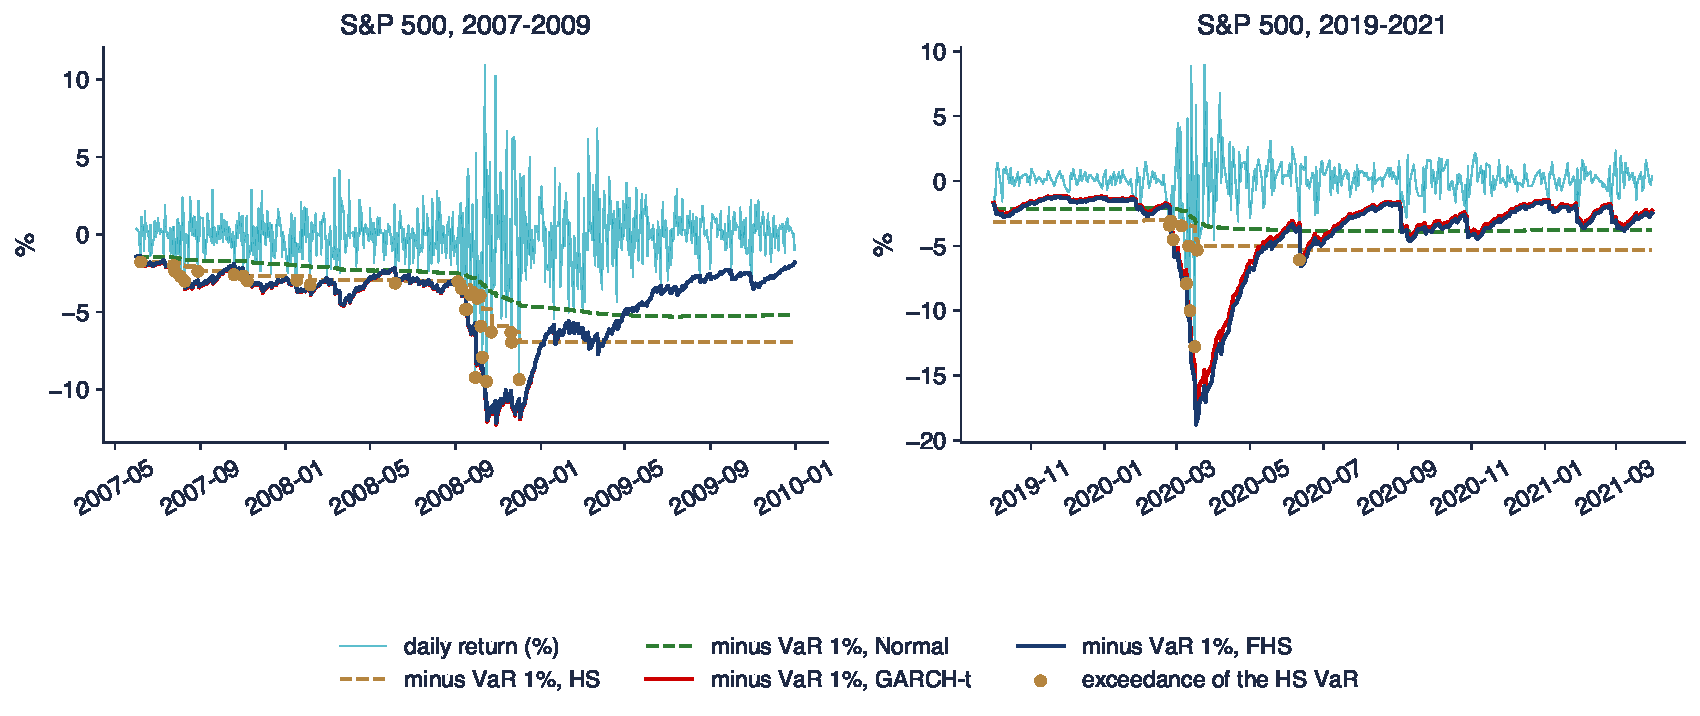
\includegraphics[width=0.97\textwidth,height=0.52\textheight,keepaspectratio]{sfm_ch10_rolling_var.pdf}
\end{center}
\vspace{-0.25cm}
\begin{itemize}
    \item S\&P 500: daily returns and minus the VaR 1\% forecasts of the four methods; dots: exceptions of the HS VaR
    \item HS and Normal react months late: the 500-day window changes slowly; GARCH-t and FHS jump within days
    \item Interpretation: after the crisis HS stays high for two years (the ghost effect), while GARCH-t returns to normal levels
\end{itemize}
\sfmquantlet{Ch_10}{SFM_ch10_conditional_var}
\end{frame}

\begin{frame}{Stress Periods: Exceptions in 2008 and 2020}
\itemsize{\footnotesize}
\begin{center}
\footnotesize
\begin{tabular}{l|rrrr|r|rrrr|r}
\toprule
& \multicolumn{5}{c|}{Sep 2008 -- Mar 2009} & \multicolumn{5}{c}{Feb -- May 2020} \\ & HS & Normal & GARCH-t & FHS & exp. & HS & Normal & GARCH-t & FHS & exp. \\
\midrule
S\&P 500 & 15 & 21 & 5 & 5 & 1.5 & 9 & 12 & 3 & 3 & 0.7 \\
DAX & 6 & 18 & 3 & 3 & 1.5 & 8 & 13 & 3 & 3 & 0.7 \\
BET & 8 & 14 & 4 & 4 & 1.4 & 5 & 10 & 4 & 4 & 0.7 \\
\bottomrule
\end{tabular}
\end{center}
\begin{itemize}
    \item Exceptions of the VaR 1\%: days with $r_t < -\mathrm{VaR}_t$; exp.: 1\% of the days in the period
    \item In 2008 the S\&P 500 Normal VaR was exceeded on 21 of 146 days, HS on 15; GARCH-t and FHS on 5
    \item Interpretation: no method is perfect in a crisis, but the conditional ones fail far less: the volatility forecast matters more than the tail shape
\end{itemize}\sfmquantlet{Ch_10}{SFM_ch10_backtesting}
\end{frame}

\begin{frame}{Which Method When?}
\itemsize{\footnotesize}
\begin{center}
\footnotesize
\begin{tabular}{>{\raggedright\arraybackslash}p{3.6cm}>{\raggedright\arraybackslash}p{3.3cm}>{\raggedright\arraybackslash}p{4.0cm}}
\toprule
\textbf{Situation} & \textbf{Method} & \textbf{Reason} \\
\midrule
daily VaR of a liquid position & GARCH-t, FHS & follow the volatility; FHS keeps the empirical tail \\
long history, quick check & HS & no model, easy to explain \\
very small $\alpha$ (0.1\%), stress tests & EVT & extrapolates beyond the worst day \\
portfolio of many assets & variance--covariance, copula & dependence; the t copula for joint crashes \\
moderate skewness and kurtosis & Cornish--Fisher & a quick correction of the Normal \\
\bottomrule
\end{tabular}
\end{center}
\begin{itemize}
    \item Never only the Normal for daily data; always report the method, the window and the level
    \item Whatever the method: backtest it (Section 7)
\end{itemize}
\end{frame}

\begin{frame}{Recap: Conditional VaR}
\itemsize{\small}
\begin{itemize}
    \item $\mathrm{VaR}_{t+1} = -(\mu + \sigma_{t+1}q_\alpha(z))$: GARCH-t (parametric $z$) or FHS (empirical $z$)
    \item Conditional VaR follows the storms; window-based VaR lags and keeps ghosts
    \item In 2008 and 2020 the conditional methods had a few times fewer exceptions
\end{itemize}
\end{frame}


%=============================================================================
\section{Portfolio VaR and Dependence}
%=============================================================================

\begin{frame}{A BET and S\&P 500 Portfolio}
\itemsize{\small}
\begin{itemize}
    \item Weights $w = (0.5, 0.5)$; simple returns $R_t$ in \%, so that $R_{p,t} = w_1R_{1,t} + w_2R_{2,t}$ exactly
    \begin{itemize}
        \item prices joined on the 6\,466 common trading days since 2000, then returns
        \item each index in its own currency: the currency risk of a RON investor is left out
    \end{itemize}
    \item Daily data: BET $\hat\mu = 0.076$, $\hat\sigma = 1.42$; S\&P 500 $\hat\mu = 0.034$, $\hat\sigma = 1.23$; correlation $\hat\rho = 0.21$
    \begin{itemize}
        \item the BVB closes before New York opens: part of the joint reaction appears one day later, so same-day correlation understates the link
    \end{itemize}
    \item Question: is the portfolio VaR smaller than the average of the two VaRs, and by how much?
\end{itemize}
\end{frame}

\begin{frame}{The Variance--Covariance Method}
\itemsize{\footnotesize}
\begin{itemize}
    \item Portfolio: $\mu_p = w^\top\mu$, $\sigma_p^2 = w^\top\Sigma w = w_1^2\sigma_1^2 + w_2^2\sigma_2^2 + 2w_1w_2\rho\sigma_1\sigma_2$ ($\Sigma$: covariance matrix)
    \begin{itemize}
        \item $w$: the vector of weights; $\mu$: the vector of mean returns; $\rho$: the correlation of the two assets
        \item if returns are jointly Normal: $\mathrm{VaR}_p = -(\mu_p + z_\alpha\sigma_p)$ (the RiskMetrics method \refRM)
    \end{itemize}
    \item \textbf{Step by step}: $\sigma_p^2 = 0.712^2 + 0.614^2 + 2 \times 0.5 \times 0.5 \times 0.369 = 1.068$, $\sigma_p = 1.033$
    \begin{itemize}
        \item VaR 1\% $= -(0.055 - 2.326 \times 1.033) = 2.35\%$; the weighted sum of the two Normal VaRs: $0.5 \times 3.23 + 0.5 \times 2.82 = 3.03\%$
        \item \textbf{diversification benefit}: 22\% of the risk disappears; with $\rho = 1$ it would be zero
    \end{itemize}
    \item Euler contributions $w_i(\Sigma w)_i/\sigma_p$ ($(\Sigma w)_i$: the $i$-th entry of $\Sigma w$) add up to $\sigma_p$: BET 56\%, S\&P 500 44\% of the portfolio risk
\end{itemize}
\end{frame}

\begin{frame}{Correlation Rises in Crises}
\itemsize{\footnotesize}
\begin{center}
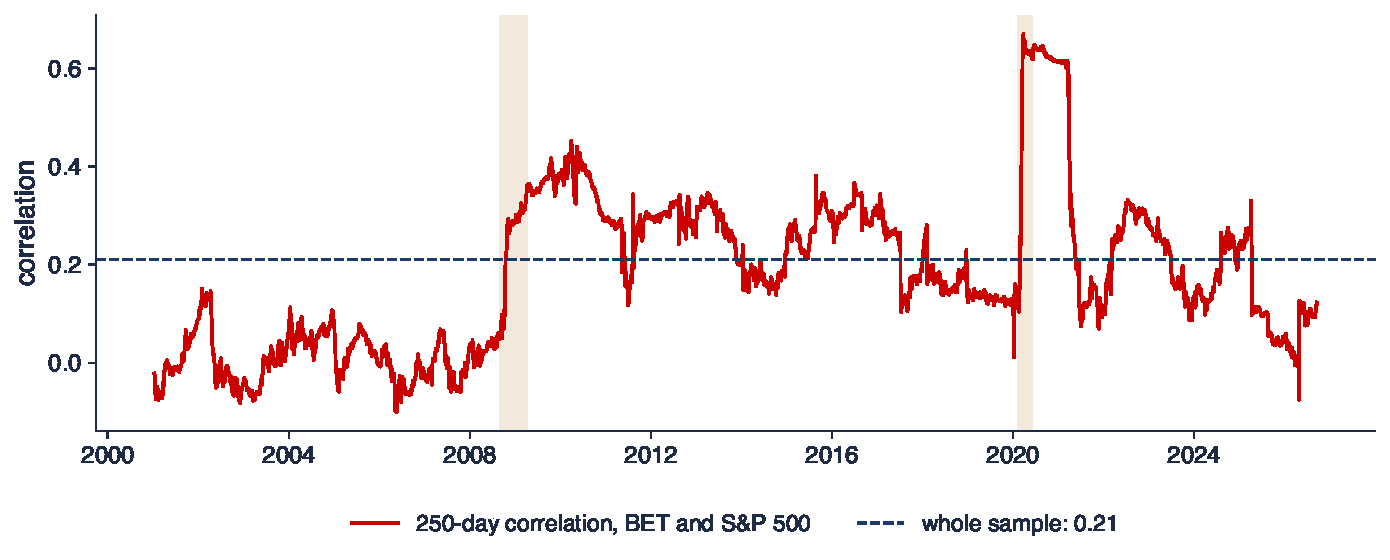
\includegraphics[width=0.97\textwidth,height=0.45\textheight,keepaspectratio]{sfm_ch10_rolling_corr.pdf}
\end{center}
\vspace{-0.25cm}
\begin{itemize}
    \item 250-day correlation of BET and S\&P 500 daily returns; shaded: the 2008 and 2020 stress periods
    \item Correlation within each period: 2017 (calm) $0.20$; Sep. 2008 -- Mar. 2009 $0.37$; Feb. -- May 2020 $0.71$
    \item Maximum of the 250-day correlation: $0.67$ on 25 March 2020
    \item Interpretation: diversification is weakest exactly when it is needed: a VaR built on the average correlation is too optimistic in a crisis
\end{itemize}
\sfmquantlet{Ch_10}{SFM_ch10_portfolio_copula}
\end{frame}

\begin{frame}{Correlation Is Not Tail Dependence}
\itemsize{\small}
\begin{itemize}
    \item Pearson correlation measures linear co-movement over all days; it is dominated by ordinary days \refEMS
    \begin{itemize}
        \item rank correlations (Spearman, Kendall's $\tau$) use only the order of the returns: Kendall $\hat\tau = 0.100$, Spearman $0.15$
    \end{itemize}
    \item \textbf{Lower tail dependence}: $\lambda_L = \lim_{q \to 0} P(U_1 \le q \mid U_2 \le q)$, $U_i = F_i(X_i)$ (the returns on a uniform scale)
    \begin{itemize}
        \item $q$: a small probability; $F_i$: the distribution function of asset $i$; $\lambda_L \in [0, 1]$
        \item the chance that BET has one of its worst days given that the S\&P 500 has one of its worst days
        \item data: $q = 5\%$: $0.22$; $q = 1\%$: $0.19$; under independence both would equal $q$
    \end{itemize}
    \item Joint crash (both below their own 1\% quantile): 0.19\% of the days, against 0.01\% under independence
\end{itemize}
\end{frame}

\begin{frame}{Copulas: a Light Introduction}
\itemsize{\small}
\begin{itemize}
    \item \textbf{Sklar's theorem}: every joint distribution function can be written as $F(x_1, x_2) = C(F_1(x_1), F_2(x_2))$ \refQRM
    \begin{itemize}
        \item $F_1$, $F_2$: the marginal distributions (each asset alone); $C$: the \textbf{copula}, a joint distribution of uniforms on $[0,1]^2$
        \item the copula holds all the dependence, the margins all the individual tails
    \end{itemize}
    \item Practical recipe
    \begin{itemize}
        \item margins: empirical or fitted (Student-t, EVT); dependence: a copula fitted to the \textbf{pseudo-observations} $\hat U_{i,t} = \mathrm{rank}(X_{i,t})/(n + 1)$
        \item simulate $(U_1, U_2)$ from the copula, map back with $F_i^{-1}$, compute the portfolio return, read VaR and ES
    \end{itemize}
    \item Textbook: \refFHH, Ch.~17
\end{itemize}
\end{frame}

\begin{frame}{Gaussian and t Copulas}
\itemsize{\footnotesize}
\begin{itemize}
    \item \textbf{Gaussian copula}: the dependence of a bivariate Normal with correlation $\rho$; $\lambda_L = 0$ for $\rho < 1$
    \begin{itemize}
        \item extreme days become independent in the limit: joint crashes are rare
    \end{itemize}
    \item \textbf{t copula}: the dependence of a bivariate Student-t with $\rho$ and $\nu$ \refDM
    \begin{itemize}
        \item $\lambda_L = 2\,t_{\nu+1}\Big(-\sqrt{(\nu + 1)(1 - \rho)/(1 + \rho)}\Big) > 0$: crashes cluster across assets
        \item $t_{\nu+1}(\cdot)$: the distribution function of a Student-t with $\nu + 1$ degrees of freedom; a smaller $\nu$ or a larger $\rho$ gives a larger $\lambda_L$
    \end{itemize}
    \item Fit on BET and S\&P 500: $\rho = \sin(\pi\hat\tau/2) = 0.157$ (valid for both copulas); $\hat\nu = 4.50$ by maximum likelihood
    \begin{itemize}
        \item log-likelihood: Gaussian $92.1$, t $219.5$; LR $= 254.9$, far above $\chi^2_{0.95}(1) = 3.84$: the t copula wins
        \item implied tail dependence $\lambda_L = 0.096$, against 0 for the Gaussian copula
    \end{itemize}
\end{itemize}
\end{frame}

\begin{frame}{Joint Bad Days: Data and Two Copulas}
\itemsize{\footnotesize}
\begin{center}
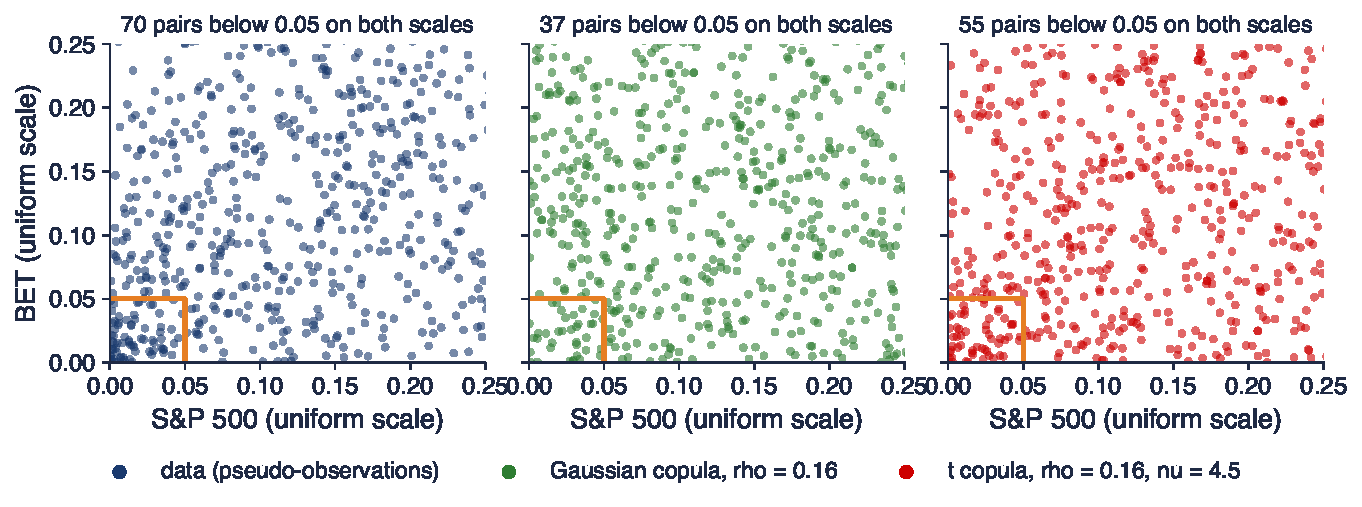
\includegraphics[width=0.97\textwidth,height=0.48\textheight,keepaspectratio]{sfm_ch10_copula.pdf}
\end{center}
\vspace{-0.25cm}
\begin{itemize}
    \item Lower-left corner of the uniform scale: pseudo-observations and samples of the same size (6\,466) from the fitted copulas
    \item Days on which both indices are among their worst 5\%: data 70, Gaussian 37, t 55; independence: about 16
    \item Interpretation: the Gaussian copula halves the number of joint bad days; the t copula is much closer to the data
\end{itemize}
\sfmquantlet{Ch_10}{SFM_ch10_portfolio_copula}
\end{frame}

\begin{frame}{Copula VaR: the Simulation Step by Step}
\itemsize{\small}
\begin{itemize}
    \item \textbf{1.} Draw $(Z_1, Z_2)$ from a bivariate Normal with correlation $\rho$
    \begin{itemize}
        \item Gaussian copula: $U_i = \Phi(Z_i)$
        \item t copula: draw $W \sim \chi^2_\nu$, set $U_i = t_\nu(Z_i\sqrt{\nu/W})$: the common factor $\sqrt{\nu/W}$ makes extremes happen together
    \end{itemize}
    \item \textbf{2.} Map to returns with the empirical quantile functions: $R_i = \hat F_i^{-1}(U_i)$
    \item \textbf{3.} Portfolio return $R_p = 0.5R_1 + 0.5R_2$; repeat 200\,000 times
    \item \textbf{4.} VaR 1\% and ES 2.5\% by historical simulation on the simulated $R_p$
    \item Same margins in both copulas: any difference in VaR comes from the dependence alone
\end{itemize}\sfmquantlet{Ch_10}{SFM_ch10_portfolio_copula}
\end{frame}

\begin{frame}{Portfolio VaR 1\% and ES 2.5\% by Method}
\itemsize{\footnotesize}
\begin{center}
\footnotesize
\begin{tabular}{lrrr}
\toprule
Method & VaR 1\% & ES 2.5\% & P(joint crash at 1\%) \\
\midrule
variance--covariance (Normal) & $2.35$ & $2.36$ & -- \\
Gaussian copula, empirical margins & $2.75$ & $2.93$ & 0.03\% \\
t copula, empirical margins & $2.81$ & $3.03$ & 0.13\% \\
historical simulation (the data) & $3.08$ & $3.30$ & 0.19\% \\
\bottomrule
\end{tabular}
\end{center}
\begin{itemize}
    \item In \%, 50/50 portfolio, 6\,466 common days; copulas: 200\,000 simulated days
    \item The Normal method misses both the heavy margins and the tail dependence; the copulas fix the margins, the t copula also the joint crashes
    \item Interpretation: the t copula still understates the historical VaR: the BET--S\&P 500 link is stronger in crises than any constant copula can describe
\end{itemize}\sfmquantlet{Ch_10}{SFM_ch10_portfolio_copula}
\end{frame}

\begin{frame}{Recap: Portfolio VaR and Dependence}
\itemsize{\small}
\begin{itemize}
    \item Variance--covariance: $\sigma_p^2 = w^\top\Sigma w$; diversification lowers VaR when $\rho < 1$
    \item Correlation rises in crises; tail dependence is what matters for joint crashes
    \item Copula = dependence on the uniform scale; the t copula has tail dependence, the Gaussian has none
\end{itemize}
\end{frame}


%=============================================================================
\section{Backtesting}
%=============================================================================

\begin{frame}{The Idea: the Hit Sequence}
\itemsize{\small}
\begin{itemize}
    \item \textbf{Exception} (hit): a day with $r_t < -\mathrm{VaR}_t$; $I_t = \mathbf{1}\{r_t < -\mathrm{VaR}_t\}$
    \begin{itemize}
        \item the VaR must be the forecast made the day before: no look-ahead
    \end{itemize}
    \item A correct VaR at level $\alpha$: the $I_t$ are i.i.d.\ Bernoulli($\alpha$) \refChris
    \begin{itemize}
        \item \textbf{unconditional coverage}: $P(I_t = 1) = \alpha$: the right number of exceptions
        \item \textbf{independence}: an exception today does not make one tomorrow more likely
    \end{itemize}
    \item Number of exceptions in $n$ days: $x = \sum_t I_t \sim \mathrm{Binomial}(n, \alpha)$, mean $n\alpha$, variance $n\alpha(1 - \alpha)$
\end{itemize}
\end{frame}

\begin{frame}{Exceptions in 250 Days under a Correct VaR 1\%}
\itemsize{\footnotesize}
\begin{center}
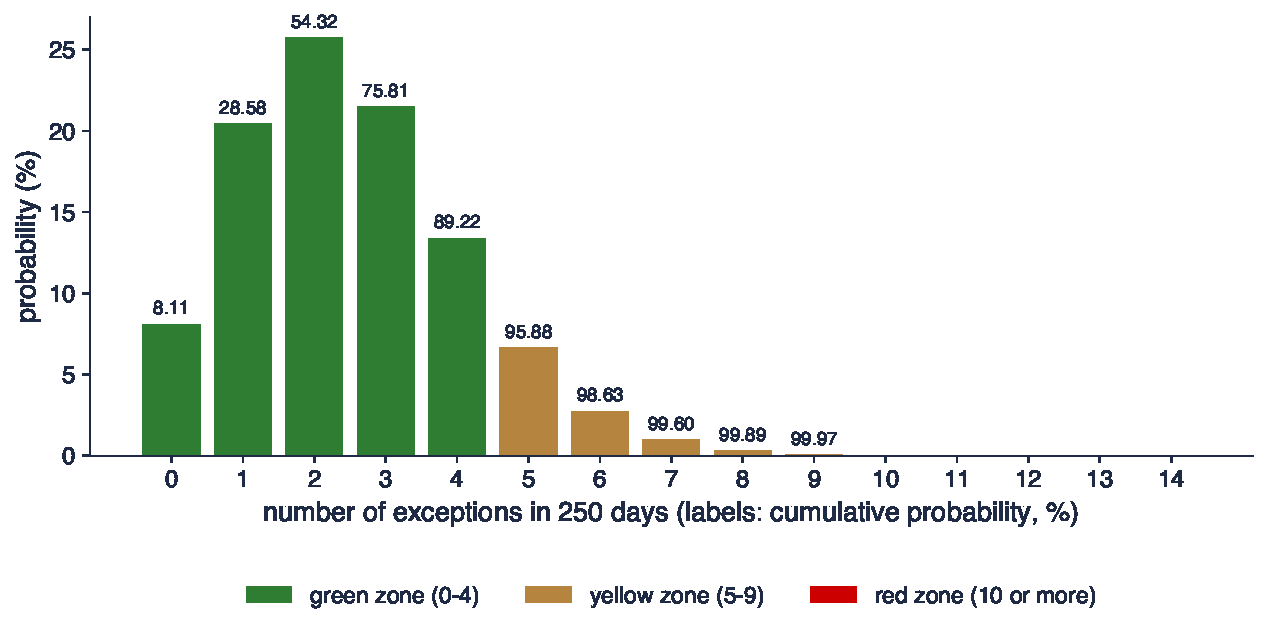
\includegraphics[width=0.97\textwidth,height=0.48\textheight,keepaspectratio]{sfm_ch10_binomial.pdf}
\end{center}
\vspace{-0.25cm}
\begin{itemize}
    \item $\mathrm{Binomial}(250, 0.01)$: expected 2.5 exceptions; 0 exceptions with probability 8.11\%, 5 or more with probability $100\% - 89.22\%$, about 11\%
    \item Interpretation: one year of data separates a good model from a bad one only roughly: a correct model lands in the yellow zone about one year in nine
\end{itemize}
\sfmquantlet{Ch_10}{SFM_ch10_backtesting}
\end{frame}

\begin{frame}{Kupiec's POF Test}
\itemsize{\footnotesize}
\begin{itemize}
    \item \textbf{POF} (proportion of failures) \refKupiec: $H_0$: $P(I_t = 1) = \alpha$; $\hat\pi = x/n$
    \begin{itemize}
        \item $LR_{uc} = -2\big[(n - x)\ln(1 - \alpha) + x\ln\alpha - (n - x)\ln(1 - \hat\pi) - x\ln\hat\pi\big] \sim \chi^2(1)$ under $H_0$
        \item $x$: exceptions in $n$ days; $\hat\pi$: the observed rate; $LR_{uc}$ compares the likelihood under the rate $\alpha$ with that under $\hat\pi$
        \item $LR_{uc} \ge 0$; a likelihood-ratio test (\sfmchlink{https://danpele.github.io/SFM/EN/Courses/chapter6_model_selection_risk_management.pdf}{Chapter 6}); reject at 5\% if $LR_{uc} > 3.84$
    \end{itemize}
    \item \textbf{Step by step}: $n = 250$, $x = 7$, $\hat\pi = 0.028$
    \begin{itemize}
        \item $\ln L_0 = 243\ln 0.99 + 7\ln 0.01 = -34.68$; $\ln L_1 = 243\ln 0.972 + 7\ln 0.028 = -31.93$
        \item $LR_{uc} = -2(-34.68 - (-31.93)) = 5.50$, p $= 0.019$: rejected at 5\%
    \end{itemize}
    \item Low power with one year of data
    \begin{itemize}
        \item in 250 days, any count from 1 to 6 is accepted at 5\%: a model with a true rate of 2\% passes with probability 76\%
        \item too few exceptions are also rejected: an overly prudent VaR wastes capital
    \end{itemize}
\end{itemize}
\end{frame}

\begin{frame}{Kupiec on 21 Years of S\&P 500 Forecasts}
\itemsize{\footnotesize}
\begin{itemize}
    \item GARCH-t VaR 1\%, 3 January 2005 -- 18 September 2026: $n = 5\,460$ days, $x = 95$ exceptions, $\hat\pi = 0.0174$
    \begin{itemize}
        \item expected $n\alpha = 55$; a 95\% binomial range for the rate under $H_0$: 0.75--1.26\%
    \end{itemize}
    \item \textbf{Step by step}
    \begin{itemize}
        \item $\ln L_0 = 5365\ln 0.99 + 95\ln 0.01 = -491.4$
        \item $\ln L_1 = 5365\ln(1 - 0.0174) + 95\ln 0.0174 = -479.0$
        \item $LR_{uc} = -2(\ln L_0 - \ln L_1) = 24.73$, p $<$\,0.001
    \end{itemize}
    \item Interpretation: with 21 years of data even a rate of 1.74\% instead of 1\% is clearly rejected; the missing leverage effect (\sfmchlink{https://danpele.github.io/SFM/EN/Courses/chapter9_arch_garch_models.pdf}{Chapter 9}) is a likely cause
\end{itemize}\sfmquantlet{Ch_10}{SFM_ch10_backtesting}
\end{frame}

\begin{frame}{Christoffersen's Independence Test}
\itemsize{\footnotesize}
\begin{itemize}
    \item Count the transitions: $n_{ij}$ = number of days with $I_{t-1} = i$ and $I_t = j$; $\hat\pi_{01} = \dfrac{n_{01}}{n_{00} + n_{01}}$, $\hat\pi_{11} = \dfrac{n_{11}}{n_{10} + n_{11}}$
    \begin{itemize}
        \item $\hat\pi_{01}$: the rate of exceptions after a day without one; $\hat\pi_{11}$: after a day with one
        \item $H_0$: $\pi_{01} = \pi_{11}$ (an exception today does not change the chance of one tomorrow) \refChris
        \item $LR_{ind} = -2\ln\dfrac{(1 - \hat\pi)^{n_{00} + n_{10}}\hat\pi^{n_{01} + n_{11}}}{(1 - \hat\pi_{01})^{n_{00}}\hat\pi_{01}^{n_{01}}(1 - \hat\pi_{11})^{n_{10}}\hat\pi_{11}^{n_{11}}} \sim \chi^2(1)$
    \end{itemize}
    \item \textbf{Conditional coverage}: $LR_{cc} = LR_{uc} + LR_{ind} \sim \chi^2(2)$; reject at 5\% if $LR_{cc} > 5.99$
    \item \textbf{Example}: S\&P 500, HS VaR 1\%, 5\,460 days: $n_{00} = 5313$, $n_{01} = 69$, $n_{10} = 69$, $n_{11} = 8$
    \begin{itemize}
        \item $\hat\pi_{01} = 1.28\%$, $\hat\pi_{11} = 10.4\%$: after an exception the next one is 8 times more likely
        \item $LR_{ind} = 19.43$ (p $<$\,0.001): the exceptions cluster
    \end{itemize}
\end{itemize}
\end{frame}

\begin{frame}{The Basel Traffic Light}
\itemsize{\footnotesize}
\begin{columns}[T]
\begin{column}{0.44\textwidth}
\begin{center}
\scriptsize
\begin{tabular}{lcrrr}
\toprule
$x$ & Zone & Cum.\ (\%) & Plus & Factor \\
\midrule
0 & green & $8.11$ & $0.00$ & $3.00$ \\
1 & green & $28.58$ & $0.00$ & $3.00$ \\
2 & green & $54.32$ & $0.00$ & $3.00$ \\
3 & green & $75.81$ & $0.00$ & $3.00$ \\
4 & green & $89.22$ & $0.00$ & $3.00$ \\
5 & yellow & $95.88$ & $0.40$ & $3.40$ \\
6 & yellow & $98.63$ & $0.50$ & $3.50$ \\
7 & yellow & $99.60$ & $0.65$ & $3.65$ \\
8 & yellow & $99.89$ & $0.75$ & $3.75$ \\
9 & yellow & $99.97$ & $0.85$ & $3.85$ \\
$\ge 10$ & red & $99.99$ & $1.00$ & $4.00$ \\
\bottomrule
\end{tabular}
\end{center}

\end{column}
\begin{column}{0.54\textwidth}
\begin{itemize}
    \item \refBCBSb: count the exceptions of the one-day VaR 1\% over the last 250 days
    \begin{itemize}
        \item green: no action; yellow: the multiplier grows by the plus factor; red: the model is presumed wrong
    \end{itemize}
    \item Capital $= (3 + \text{plus}) \times$ the 60-day average of the 10-day VaR 1\% (or yesterday's value, if larger)
    \begin{itemize}
        \item zones from the binomial: yellow starts where the cumulative probability first exceeds 95\%, red where it reaches 99.99\%
    \end{itemize}
    \item $x$: exceptions in 250 days; Cumul.: $P(X \le x)$ under $\mathrm{Binomial}(250, 0.01)$
    \item FRTB keeps the count of VaR 1\% exceptions at bank and desk level \refMARb
\end{itemize}
\end{column}
\end{columns}
\end{frame}

\begin{frame}{When Do the Exceptions Happen?}
\itemsize{\footnotesize}
\begin{center}
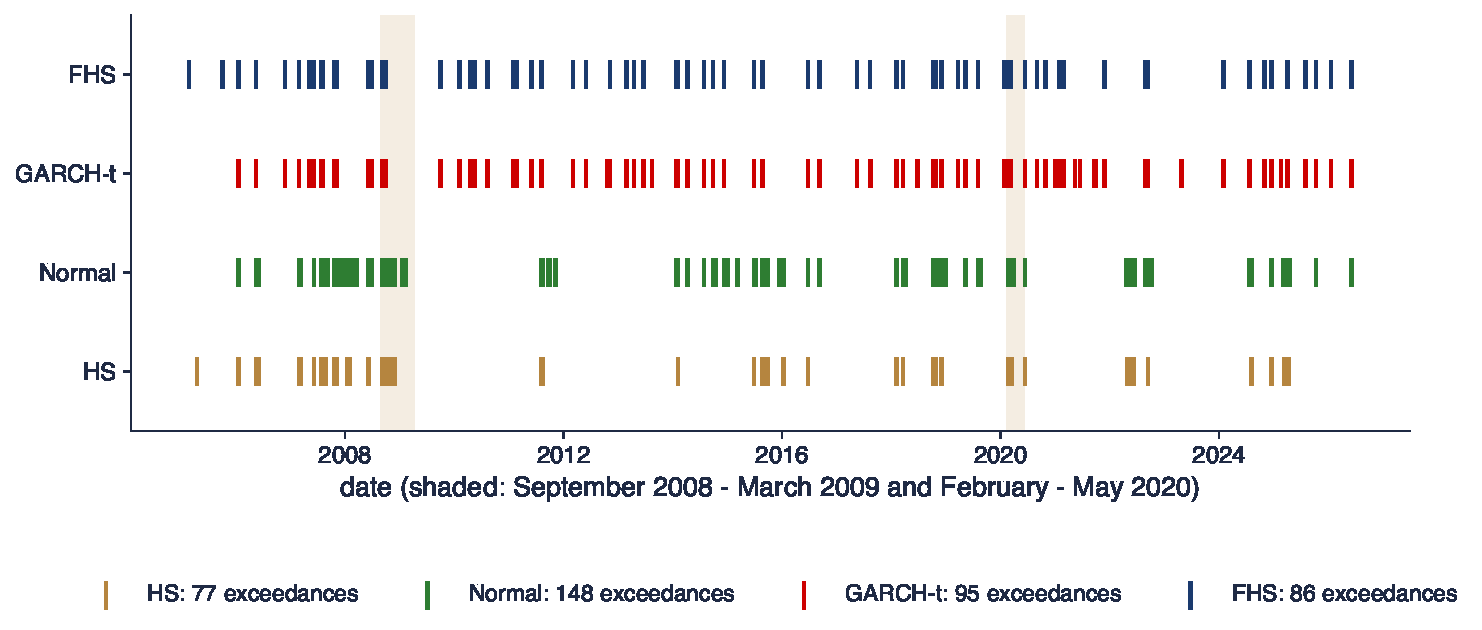
\includegraphics[width=0.97\textwidth,height=0.48\textheight,keepaspectratio]{sfm_ch10_hits.pdf}
\end{center}
\vspace{-0.25cm}
\begin{itemize}
    \item S\&P 500, 2005--2026: each mark is a day on which the VaR 1\% of the method was exceeded; expected about 55 per method
    \item Interpretation: HS and Normal exceptions come in bursts (2007--2008, 2011, 2022); GARCH-t and FHS exceptions are spread over time, but there are more of them in calm years
\end{itemize}
\sfmquantlet{Ch_10}{SFM_ch10_backtesting}
\end{frame}

\begin{frame}{Backtest Results: S\&P 500 and DAX}
\itemsize{\footnotesize}
\begin{center}
\scriptsize
\begin{tabular}{llrrrrrrr}
\toprule
& Method & $x$ & rate (\%) & p POF & p ind. & p c.c. & max 250 d. & $Z_2$ (p) \\
\midrule
S\&P 500 & HS & 77 & $1.41$ & 0.004 & $<$\,0.001 & $<$\,0.001 & 18 & ${-0.39}$ ($<$\,0.001) \\
 & Normal & 148 & $2.71$ & $<$\,0.001 & $<$\,0.001 & $<$\,0.001 & 29 & ${-1.15}$ ($<$\,0.001) \\
 & GARCH-t & 95 & $1.74$ & $<$\,0.001 & 0.114 & $<$\,0.001 & 10 & ${-0.54}$ ($<$\,0.001) \\
 & FHS & 86 & $1.58$ & $<$\,0.001 & 0.060 & $<$\,0.001 & 10 & ${-0.20}$ (0.013) \\
\midrule
DAX & HS & 67 & $1.21$ & 0.121 & $<$\,0.001 & $<$\,0.001 & 12 & ${-0.26}$ (0.002) \\
 & Normal & 133 & $2.41$ & $<$\,0.001 & $<$\,0.001 & $<$\,0.001 & 19 & ${-0.87}$ ($<$\,0.001) \\
 & GARCH-t & 84 & $1.52$ & $<$\,0.001 & 0.549 & 0.001 & 9 & ${-0.49}$ ($<$\,0.001) \\
 & FHS & 77 & $1.40$ & 0.005 & 0.418 & 0.015 & 9 & ${-0.18}$ (0.014) \\
\bottomrule
\end{tabular}
\end{center}
\begin{itemize}
    \item VaR 1\% since 3 January 2005 (about 5\,500 days); $x$: exceptions; p ind.: Christoffersen independence; p c.c.: conditional coverage; max 250 d.: the worst 250-day count
    \item Normal: rejected everywhere; HS: exceptions cluster; GARCH-t and FHS: independent exceptions, but a rate of 1.4--1.7\%
\end{itemize}\sfmquantlet{Ch_10}{SFM_ch10_backtesting}
\end{frame}

\begin{frame}{Backtest Results: BET and Bitcoin}
\itemsize{\footnotesize}
\begin{center}
\scriptsize
\begin{tabular}{llrrrrrrr}
\toprule
& Method & $x$ & rate (\%) & p POF & p ind. & p c.c. & max 250 d. & $Z_2$ (p) \\
\midrule
BET & HS & 66 & $1.22$ & 0.123 & 0.001 & 0.002 & 14 & ${-0.27}$ (0.001) \\
 & Normal & 122 & $2.25$ & $<$\,0.001 & $<$\,0.001 & $<$\,0.001 & 21 & ${-0.83}$ ($<$\,0.001) \\
 & GARCH-t & 65 & $1.20$ & 0.158 & 0.807 & 0.358 & 9 & ${-0.22}$ (0.007) \\
 & FHS & 65 & $1.20$ & 0.158 & 0.240 & 0.185 & 7 & ${-0.18}$ (0.021) \\
\midrule
Bitcoin & HS & 33 & $0.93$ & 0.672 & 0.316 & 0.553 & 6 & ${-0.07}$ (0.224) \\
 & Normal & 69 & $1.94$ & $<$\,0.001 & 0.057 & $<$\,0.001 & 16 & ${-0.56}$ ($<$\,0.001) \\
 & GARCH-t & 48 & $1.35$ & 0.045 & 0.683 & 0.123 & 8 & ${-0.41}$ ($<$\,0.001) \\
 & FHS & 24 & $0.68$ & 0.040 & 0.155 & 0.044 & 6 & ${0.12}$ (0.834) \\
\bottomrule
\end{tabular}
\end{center}
\begin{itemize}
    \item VaR 1\% since 3 January 2005 (Bitcoin since 1 January 2017); $x$: exceptions; p ind.: Christoffersen independence; p c.c.: conditional coverage; max 250 d.: the worst 250-day count
    \item BET: GARCH-t and FHS pass all three tests; Bitcoin: HS passes, FHS is too prudent ($0.68\%$)
\end{itemize}\sfmquantlet{Ch_10}{SFM_ch10_backtesting}
\end{frame}

\begin{frame}{Ranking the Forecasts, and Today's Zone}
\itemsize{\footnotesize}
\begin{center}
\footnotesize
\begin{tabular}{l|rrrr|rrrr}
\toprule
& \multicolumn{4}{c|}{average quantile loss $\times 100$} & \multicolumn{4}{c}{exceptions, last 250 days} \\ & HS & Normal & GARCH-t & FHS & HS & Normal & GARCH-t & FHS \\
\midrule
S\&P 500 & $5.17$ & $5.80$ & $3.71$ & $3.68$ & 0 & 2 & 3 & 3 \\
DAX & $5.15$ & $5.52$ & $4.08$ & $4.05$ & 1 & 3 & 3 & 3 \\
BET & $6.04$ & $6.26$ & $4.59$ & $4.62$ & 4 & 6 & 3 & 2 \\
Bitcoin & $13.57$ & $14.52$ & $13.53$ & $13.75$ & 3 & 4 & 2 & 2 \\
\bottomrule
\end{tabular}
\end{center}
\begin{itemize}
    \item Tests say whether a model is acceptable; a \textbf{scoring function} says which of two models is better
    \begin{itemize}
        \item VaR is elicitable: the average quantile loss $\frac1n\sum_t(\alpha - I_t)(r_t + \mathrm{VaR}_t)$ ranks the forecasts \refGneiting
    \end{itemize}
    \item The equity indices: GARCH-t and FHS have the smallest loss, the Normal the largest; Bitcoin: the four methods are close
    \item Interpretation: on the last 250 days every model is in the green zone except the Normal VaR of the BET (6, yellow): a recent window says little about a model
\end{itemize}\sfmquantlet{Ch_10}{SFM_ch10_backtesting}
\end{frame}

\begin{frame}{The Traffic Light through Time}
\itemsize{\footnotesize}
\begin{center}
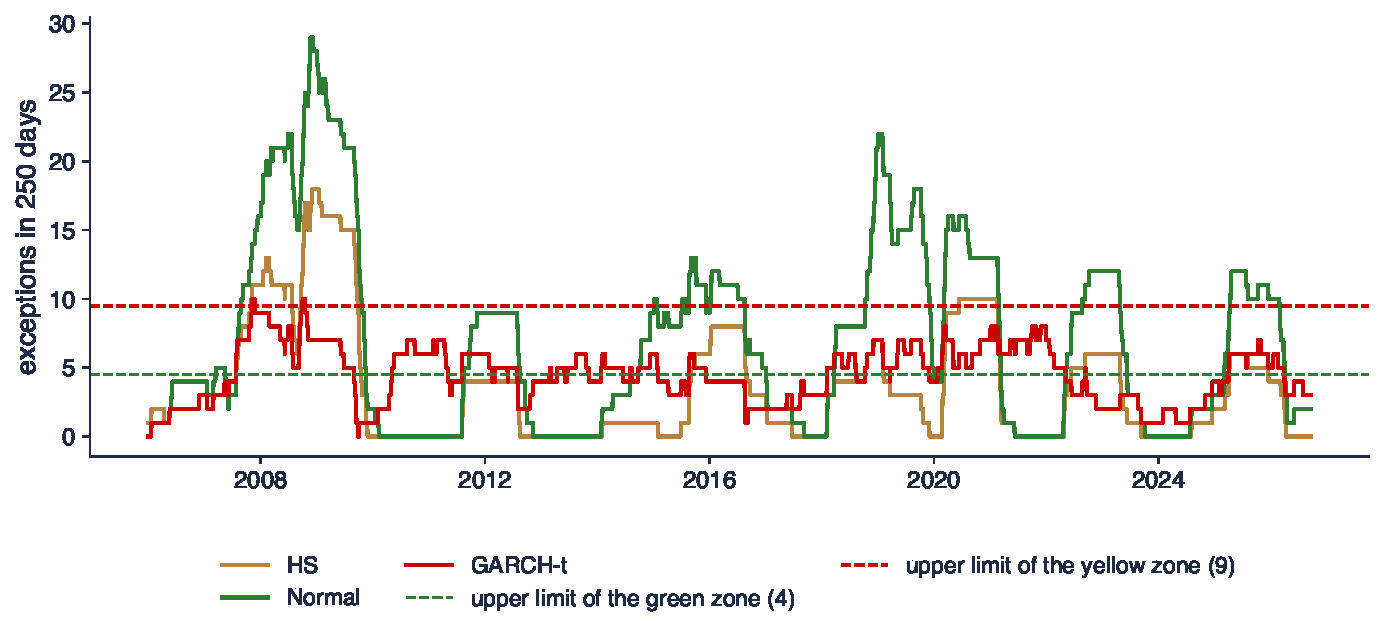
\includegraphics[width=0.97\textwidth,height=0.48\textheight,keepaspectratio]{sfm_ch10_traffic_time.pdf}
\end{center}
\vspace{-0.25cm}
\begin{itemize}
    \item S\&P 500: number of VaR 1\% exceptions in the last 250 days, for every day since 2006; dashed: the zone limits
    \item Share of days in the red zone: Normal 33\%, HS 12\%, GARCH-t 0\%; worst count: 29, 18 and 10
    \item Interpretation: a bank using the Normal or HS VaR would have paid the red-zone penalty for most of 2008--2009; GARCH-t almost never reaches the red zone
\end{itemize}
\sfmquantlet{Ch_10}{SFM_ch10_backtesting}
\end{frame}

\begin{frame}{Backtesting ES: Acerbi and Székely}
\itemsize{\footnotesize}
\begin{itemize}
    \item ES is not elicitable alone, but it can be tested together with VaR \refAS
    \begin{itemize}
        \item $Z_2 = \dfrac{1}{T\alpha}\displaystyle\sum_{t=1}^{T}\dfrac{r_t I_t}{\mathrm{ES}_t} + 1$, \quad $I_t = \mathbf{1}\{r_t < -\mathrm{VaR}_t\}$, $\alpha = 2.5\%$
        \item $T$: the number of test days; $\mathrm{VaR}_t$, $\mathrm{ES}_t$: the forecasts for day $t$; each exception adds $r_t/\mathrm{ES}_t$
        \item if VaR and ES are right, $E[Z_2] = 0$; $Z_2 < 0$: the losses beyond VaR are larger than the forecast ES, or too frequent
    \end{itemize}
    \item p-value by simulation: draw returns from each day's forecast distribution, recompute $Z_2$ 1000 times
    \begin{itemize}
        \item S\&P 500: Normal $Z_2 = -1.15$, HS $-0.39$, GARCH-t $-0.54$, FHS $-0.20$ (p 0.013)
    \end{itemize}
    \item Interpretation: all four ES 2.5\% forecasts are too small for the equity indices; FHS is closest, because it takes the tail of $z$ from the data
\end{itemize}\sfmquantlet{Ch_10}{SFM_ch10_backtesting}
\end{frame}

\begin{frame}{Case Study: VaR Models at Commercial Banks}
\itemsize{\small}
\begin{itemize}
    \item \refBO: the first study of the VaR forecasts that large US banks actually reported, with their daily trading P\&L
    \begin{itemize}
        \item design: the banks' VaR 1\% against the realised P\&L; a simple GARCH model of each bank's P\&L as the benchmark
    \end{itemize}
    \item Findings
    \begin{itemize}
        \item the banks' VaR was conservative on average, yet the exceptions that did occur came in clusters
        \item the GARCH benchmark gave lower VaRs with comparable coverage: it followed changes in volatility better
    \end{itemize}
    \item The same pattern as in our data: window-based VaR is either too high in calm times or too slow in storms; conditional VaR adapts
    \item Further reading on forecasting the quantile directly: CAViaR \refCAViaR
\end{itemize}
\end{frame}

\begin{frame}{Recap: Backtesting}
\itemsize{\small}
\begin{itemize}
    \item Exceptions should be Bernoulli($\alpha$) and independent: Kupiec tests the rate, Christoffersen the clustering
    \item Basel traffic light: 0--4 green, 5--9 yellow, 10 or more red in 250 days
    \item ES is tested with VaR ($Z_2$); conditional methods pass more often than window methods
\end{itemize}
\end{frame}


%=============================================================================
\section{AI for Scientific Discovery}
%=============================================================================

\begin{frame}{An Open Question}
\itemsize{\small}
\begin{itemize}
    \item \textbf{Does the tail dependence between the BVB and world markets jump in crises, and does it come back?}
    \begin{itemize}
        \item today: correlation $0.20$ in a calm year, $0.71$ in spring 2020; a constant t copula gives $\lambda_L = 0.096$
        \item a portfolio VaR with a constant copula is still below the historical one (previous section)
    \end{itemize}
    \item Why it is open: crises are few, the BVB trades at other hours, and tail estimates need many observations
    \item Related work on entropy as a risk measure, as further reading: \refPeleA; \refPeleB
    \item AI tools can speed up such a study, but its results must still be checked \refWang
\end{itemize}
\end{frame}

\begin{frame}{How AI Could Help}
\itemsize{\small}
\begin{itemize}
    \item \textbf{Literature}: a list of studies on time-varying copulas and on contagion between emerging and developed markets
    \item \textbf{Code}: a first draft of rolling t-copula estimates (250 days) for BET and S\&P 500, with $\rho$, $\nu$ and $\lambda_L$ over time
    \item \textbf{Robustness}: two-day returns (different trading hours), DAX instead of S\&P 500, other windows
    \item Example prompt
    \begin{itemize}
        \item \aiprompt{Write Python code that fits a bivariate t copula by maximum likelihood to the pseudo-observations of daily BET and S\&P 500 returns on rolling windows of 250 days moved by 21 days, and plots rho, nu and the lower tail dependence over time.}
    \end{itemize}
\end{itemize}
\end{frame}

\begin{frame}{What to Check}
\itemsize{\small}
\begin{itemize}
    \item The VaR convention: ``VaR 1\%'' is the loss exceeded with probability 1\%, a positive number; an answer that names the complementary probability or reports a negative VaR mixes conventions
    \item Prices joined on common days before computing returns; the BVB and New York trade at different hours
    \item Pseudo-observations: ranks divided by $n + 1$, not by $n$ (otherwise the copula density is infinite at 1)
    \item Tail dependence from 250 days rests on a handful of joint bad days: report its uncertainty (bootstrap, \sfmchlink{https://danpele.github.io/SFM/EN/Courses/chapter2_classical_distributions_stylised_facts.pdf}{Chapter 2})
    \item Overlapping windows: consecutive estimates are not independent evidence
    \item References: every cited paper must exist; check the DOI
\end{itemize}
\end{frame}

\begin{frame}{Project Idea}
\itemsize{\small}
\begin{itemize}
    \item \textbf{Question}: does a time-varying copula give a better portfolio VaR for a BVB and world-equity portfolio than a constant one?
    \begin{itemize}
        \item data: BET, BET-TR, S\&P 500, DAX since 2005 (EODHD)
    \end{itemize}
    \item Steps
    \begin{itemize}
        \item GARCH-t margins for each index (\sfmchlink{https://danpele.github.io/SFM/EN/Courses/chapter9_arch_garch_models.pdf}{Chapter 9}); constant and rolling t copula for the dependence
        \item one-day VaR 1\% and ES 2.5\% of a 50/50 portfolio, out of sample since 2008
        \item Kupiec, Christoffersen and $Z_2$ for both versions, with special attention to 2008, 2020 and 2022
    \end{itemize}
    \item Deliverable: one table, one chart, and a paragraph on what the data can and cannot show
    \item Declare any AI use, and list the errors of the AI that you corrected
\end{itemize}
\end{frame}


%=============================================================================
\section{Summary}
%=============================================================================

\begin{frame}{Key Takeaways}
\itemsize{\small}
\begin{itemize}
    \item VaR 1\% $= -q_{1\%}$: the loss exceeded on one day in a hundred; ES 2.5\%: the average loss on the worst 2.5\% of days
    \item ES is coherent; VaR can penalise diversification; VaR is elicitable, ES only together with VaR
    \item The Normal VaR is 14--24\% too low on daily data; HS, Student-t and EVT agree at 1\%; Cornish--Fisher fails for large kurtosis
    \item Conditional VaR (GARCH-t, FHS) follows the storms and passes backtests that window methods fail
    \item Portfolio risk: correlation rises in crises; tail dependence (t copula) matters for joint crashes
    \item Backtest with Kupiec (rate), Christoffersen (clustering), the traffic light (regulation) and $Z_2$ (ES)
\end{itemize}
\end{frame}

\begin{frame}{Key Formulas}
\itemsize{\small}
{\renewcommand{\arraystretch}{1.45}\begin{center}
\small
\begin{tabular}{ll}
\toprule
\textbf{Quantity} & \textbf{Formula} \\
\midrule
VaR & $\mathrm{VaR}_\alpha = -q_\alpha(X)$; \ HS: $-r_{(\lceil n\alpha\rceil)}$ \\
ES & $\mathrm{ES}_\alpha = -\frac{1}{\alpha}\int_0^\alpha q_u\,du$; \ HS: $-\frac1k\sum_{i \le k} r_{(i)}$ \\
Normal & $-(\mu + \sigma z_\alpha)$, \ $-\mu + \sigma\varphi(z_\alpha)/\alpha$ \\
EVT (POT) & $u + \frac{\beta}{\xi}[(n\alpha/N_u)^{-\xi} - 1]$, \ ES $= (\mathrm{VaR} + \beta - \xi u)/(1 - \xi)$ \\
Conditional & $-(\mu + \sigma_{t+1}q_\alpha(z))$ \\
Portfolio & $\sigma_p^2 = w^\top\Sigma w$ \\
t copula & $\lambda_L = 2t_{\nu+1}(-\sqrt{(\nu + 1)(1 - \rho)/(1 + \rho)})$ \\
Kupiec & $LR_{uc} = -2\ln[(1-\alpha)^{n-x}\alpha^x/((1-\hat\pi)^{n-x}\hat\pi^x)] \sim \chi^2(1)$ \\
Christoffersen & $LR_{cc} = LR_{uc} + LR_{ind} \sim \chi^2(2)$ \\
Acerbi--Székely & $Z_2 = \frac{1}{T\alpha}\sum_t r_tI_t/\mathrm{ES}_t + 1$ \\
\bottomrule
\end{tabular}
\end{center}
}
\end{frame}

\begin{frame}{Check Yourself}
\itemsize{\small}
\begin{itemize}
    \item \textbf{Question}: a desk reports ``VaR 1\% = $-2.4\%$''. What is wrong?
    \begin{itemize}
        \item \textbf{Answer}: the sign: $-2.4\%$ is the 1\% quantile $q_{0.01}$; VaR 1\% $= -q_{0.01} = 2.4\%$, a loss
    \end{itemize}
    \item \textbf{Question}: a model has 3 exceptions in 250 days, all in the same week. Which test detects the problem?
    \begin{itemize}
        \item \textbf{Answer}: not Kupiec (3 is close to 2.5), but Christoffersen's independence test
    \end{itemize}
    \item \textbf{Question}: two portfolios have the same VaR 1\%. Can their ES 2.5\% differ?
    \begin{itemize}
        \item \textbf{Answer}: yes: ES depends on the whole tail beyond the quantile, VaR only on one point
    \end{itemize}
    \item Next: \sfmchlink{https://danpele.github.io/SFM/EN/Courses/chapter11_fractal_markets_long_memory.pdf}{Chapter 11}, the fractal markets hypothesis and long memory
\end{itemize}
\end{frame}


%=============================================================================
\section{References}
%=============================================================================

\begin{frame}{References (1/2)}
\itemsize{\tiny}
\begin{itemize}
    \item Acerbi, C., Székely, B. (2014). \href{https://www.msci.com/documents/10199/22aa9922-f874-4060-b77a-0f0e267a489b}{Backtesting expected shortfall}. MSCI Research; published in \textit{Risk}, December 2014.
    \item Acerbi, C., Tasche, D. (2002). \href{https://doi.org/10.1016/S0378-4266(02)00283-2}{On the coherence of expected shortfall}. \textit{Journal of Banking \& Finance}, 26(7), 1487--1503.
    \item Artzner, P., Delbaen, F., Eber, J.-M., Heath, D. (1999). \href{https://doi.org/10.1111/1467-9965.00068}{Coherent measures of risk}. \textit{Mathematical Finance}, 9(3), 203--228.
    \item Barone-Adesi, G., Giannopoulos, K., Vosper, L. (1999). \href{https://doi.org/10.1002/(SICI)1096-9934(199908)19:5<583::AID-FUT5>3.0.CO;2-S}{VaR without correlations for portfolios of derivative securities}. \textit{Journal of Futures Markets}, 19(5), 583--602.
    \item Basel Committee on Banking Supervision (1996a). \href{https://www.bis.org/publ/bcbs24.htm}{Amendment to the capital accord to incorporate market risks}. Bank for International Settlements.
    \item Basel Committee on Banking Supervision (1996b). \href{https://www.bis.org/publ/bcbs22.htm}{Supervisory framework for the use of ``backtesting'' in conjunction with the internal models approach to market risk capital requirements}. Bank for International Settlements.
    \item Basel Committee on Banking Supervision (2019). \href{https://www.bis.org/bcbs/publ/d457.htm}{Minimum capital requirements for market risk}. Bank for International Settlements.
    \item Berkowitz, J., O'Brien, J. (2002). \href{https://doi.org/10.1111/1540-6261.00455}{How accurate are value-at-risk models at commercial banks?} \textit{Journal of Finance}, 57(3), 1093--1111.
    \item Bollerslev, T. (1986). \href{https://doi.org/10.1016/0304-4076(86)90063-1}{Generalized autoregressive conditional heteroskedasticity}. \textit{Journal of Econometrics}, 31(3), 307--327.
    \item Borak, S., Härdle, W.K., López-Cabrera, B. (2013). \href{https://doi.org/10.1007/978-3-642-33929-5}{\textit{Statistics of Financial Markets: Exercises and Solutions}}, 2nd ed. Springer.
    \item Christoffersen, P.F. (1998). \href{https://doi.org/10.2307/2527341}{Evaluating interval forecasts}. \textit{International Economic Review}, 39(4), 841--862.
    \item Cornish, E.A., Fisher, R.A. (1938). \href{https://doi.org/10.2307/1400905}{Moments and cumulants in the specification of distributions}. \textit{Revue de l'Institut International de Statistique}, 5(4), 307--320.
    \item Daníelsson, J., Jorgensen, B.N., Samorodnitsky, G., Sarma, M., de Vries, C.G. (2013). \href{https://doi.org/10.1016/j.jeconom.2012.08.011}{Fat tails, VaR and subadditivity}. \textit{Journal of Econometrics}, 172(2), 283--291.
    \item Demarta, S., McNeil, A.J. (2005). \href{https://doi.org/10.1111/j.1751-5823.2005.tb00254.x}{The t copula and related copulas}. \textit{International Statistical Review}, 73(1), 111--129.
    \item Embrechts, P., McNeil, A.J., Straumann, D. (2002). \href{https://doi.org/10.1017/CBO9780511615337.008}{Correlation and dependence in risk management: properties and pitfalls}. In M. Dempster (ed.), \textit{Risk Management: Value at Risk and Beyond}, 176--223. Cambridge University Press.
    \item Engle, R.F., Manganelli, S. (2004). \href{https://doi.org/10.1198/073500104000000370}{CAViaR: conditional autoregressive value at risk by regression quantiles}. \textit{Journal of Business \& Economic Statistics}, 22(4), 367--381.
\end{itemize}
\end{frame}

\begin{frame}{References (2/2)}
\itemsize{\tiny}
\begin{itemize}
    \item Fissler, T., Ziegel, J.F. (2016). \href{https://doi.org/10.1214/16-AOS1439}{Higher order elicitability and Osband's principle}. \textit{Annals of Statistics}, 44(4), 1680--1707.
    \item Franke, J., Härdle, W.K., Hafner, C.M. (2019). \href{https://doi.org/10.1007/978-3-030-13751-9}{\textit{Statistics of Financial Markets: An Introduction}}, 5th ed. Springer.
    \item Gneiting, T. (2011). \href{https://doi.org/10.1198/jasa.2011.r10138}{Making and evaluating point forecasts}. \textit{Journal of the American Statistical Association}, 106(494), 746--762.
    \item Hull, J., White, A. (1998). \href{https://doi.org/10.21314/JOR.1998.001}{Incorporating volatility updating into the historical simulation method for value-at-risk}. \textit{Journal of Risk}, 1(1), 5--19.
    \item J.P. Morgan/Reuters (1996). \href{https://www.msci.com/documents/10199/5915b101-4206-4ba0-aee2-3449d5c7e95a}{\textit{RiskMetrics -- Technical Document}}, 4th ed. New York.
    \item Kupiec, P.H. (1995). \href{https://doi.org/10.3905/jod.1995.407942}{Techniques for verifying the accuracy of risk measurement models}. \textit{Journal of Derivatives}, 3(2), 73--84.
    \item McNeil, A.J., Frey, R. (2000). \href{https://doi.org/10.1016/S0927-5398(00)00012-8}{Estimation of tail-related risk measures for heteroscedastic financial time series: an extreme value approach}. \textit{Journal of Empirical Finance}, 7(3--4), 271--300.
    \item McNeil, A.J., Frey, R., Embrechts, P. (2015). \href{https://press.princeton.edu/books/hardcover/9780691166278/quantitative-risk-management}{\textit{Quantitative Risk Management: Concepts, Techniques and Tools}}, revised ed. Princeton University Press.
    \item Pele, D.T., Lazar, E., Dufour, A. (2017). \href{https://doi.org/10.3390/e19050226}{Information entropy and measures of market risk}. \textit{Entropy}, 19(5), 226.
    \item Pele, D.T., Mazurencu-Marinescu-Pele, M. (2019). \href{https://doi.org/10.3390/e21020102}{Using high-frequency entropy to forecast Bitcoin's daily value at risk}. \textit{Entropy}, 21(2), 102.
    \item Wang, H., Fu, T., Du, Y., Gao, W., et al. (2023). \href{https://doi.org/10.1038/s41586-023-06221-2}{Scientific discovery in the age of artificial intelligence}. \textit{Nature}, 620, 47--60.
\end{itemize}
\end{frame}

\end{document}
